
\def\>{\rangle}
\def\<{\langle}

%\DeclareMathOperator{\mix}{mix}
%\DeclareMathOperator{\component}{comp}
%\DeclareMathOperator{\cospan}{cospan}
\newcommand\mix{\mathrm{mix}}
\newcommand\component{\mathrm{comp}}
\newcommand\cospan{\mathrm{cospan}}
\newcommand\dist{\mathrm{dist}}
\newcommand\hull{\mathrm{hull}}
\newcommand\support{\mathrm{supp}}
\newcommand\capacity{\mathrm{efc}}
\newcommand\size{\mathrm{frac}}
\newcommand\fcap{\mathrm{fcap}}

\newcommand\vspan{\mathrm{span}}
\newcommand\cl{\mathrm{cl}}

\def\distinct{\downmodels}
\def\ndistinct{\ndownmodels}
\def\disjunct{\perp}

\newcommand{\ens}[1][e] {\mathsf{#1}} % Ensemble
\newcommand{\Ens}[1][E] {\mathcal{#1}} % Ensemble space

\chapter{Ensemble spaces}

Here we summarize the work in progress for a general theory of states and processes that is applicable to any physical system. The core concept is that of an ensemble, and the goal is to find necessary requirements for ensembles that can serve as basic axioms and then further suitable assumptions to recover the different theories (e.g. classical, quantum and thermodynamics).

By ensemble we mean what is usually meant in statistical mechanics: we have a preparation device that follow some known recipe; its output is somewhat varied by it is consistently varied (i.e. its statistical properties are well defined); the collection of all possible outputs taken as one object is an ensemble. Typically, one defines statistical ensembles on top of the space of ``true'' physical states (e.g. microstates, pure states, ...). Here we will do the opposite: we will start from the ensembles and recover the states as the ``most pure'' ensembles.

The idea is that physical theories are, and can only be, about ensembles. At a practical level, most of the time we can only prepare and measure statistical properties as we do not have perfect control over any system (i.e. all measurements are really statistical). The cases where properties can be prepared with one hundred percent reliability can still be understood as ensembles of identical preparations, were the variability is limited to external conditions or internal dynamics. At a conceptual level, the goal of physics is to write laws that apply all the time: every time that one prepares a system according to a particular procedure, lets it evolve in particular conditions, he will obtain a particular result. That is, the idea of repeatability of experimental results implicitly assumes that the objects of scientific inquiry are not single instances, but the infinite collections of all reproducible instances.

Note: all $\log$s are assumed in base 2.

\section{Axiom of ensemble and topology}

The first property of ensembles is that they must be definable experimentally. As shows in the previous chapters, this means that they must form a topological space where the topology corresponds to that defined by the verifiable statements.

\begin{mathSection}
	\begin{axiom}[Axiom of ensembles] 
		The state of a system is represented by an \textbf{ensemble}, which represents all possible preparations of equivalent systems prepared according to the same procedure. The set of all possible ensembles for a particular system is an \textbf{ensemble space}. Formally, an ensemble space is a $T_0$ second countable topological space where each element is called an ensemble.
	\end{axiom}
	
	\begin{justification}
		In physics, ensembles are usually defined as probability distributions over states. This is conceptually problematic. Any actual physical preparation is always associated with some uncertainty. That is, the system will never be replicated exactly. This is true even in quantum mechanics: while we can always prepare a hydrogen atom in the ground state, we can never prepare an atom in the same exact position with the same exact velocity. The ability to prepare ensembles in which the position and the excitation of the atom can be assumed to be uncorrelated is what allows us to concentrate on one of the properties. Therefore, ensembles are the only thing that can actually be prepared in practice. Pure states, then, should not be taken as primitive notions but should be understood as an idealized ensemble. 
		
		From a more conceptual level, reproducibility is baked into the requirement of experimental verifiability. A physical law, then, must be understood as describing a relationship that always exist whenever the same set of circumstances is replicated. Given that we need to always be able to replicate those circumstances ``one more time'', the relationship is about countably infinite similar preparations: an ensemble. Therefore, to the extent that physics is about reproducible experimental results, the basic description of a system is in terms of ensembles. This justifies the use of ensembles as the fundamental object to describe the state of a system.\footnote{Note that reproducibility also already implies that all properties that characterize an ensemble must be relative to the procedure. If the properties depended, for example, on absolute space or absolute time, then different practitioners would not be able to prepare the same ensemble.}
		
		Ensembles are experimentally defined objects, and therefore they are possibilities of an experimental domain. Therefore an ensemble space is a $T_0$ second countable topological space where each element is an ensemble and the topology is induced by the verifiable statements.
	\end{justification}
\end{mathSection}

We give three canonical examples, which we aim to fully characterize within the general theory. These corresponds to the classical discrete, classical continuum and quantum ensemble spaces. Here we review these cases and give the appropriate mathematical definitions, highlighting potential issues, as these serve as models and examples for a general theory.

\subsection{Discrete classical theory}

%TODO: divide the discussion of the example to discuss topology/convex structure/entropy separately?

\begin{defn}
	The ensemble space of a \textbf{discrete classical theory} is a simplex with the standard convex structure and the Shannon entropy. The simplex can have finitely or countably many vertices.
	
	That is, a discrete classical ensemble space is a set $\Ens$ containing $n$ points $\{s_i\}^n_{i=1}$ and for which every element $\ens \in \Ens$ is characterized by a unique convex combination $\ens = \sum_i p_i s_i$ such that $\sum_i p_i = 1$. The space is closed under convex combinations of finitely many elements. The entropy is given by $S(\ens) = - \sum_i p_i \log p_i$.
\end{defn}

\begin{remark}
	The correct closure under convex combinations of countably many elements is not clear.
\end{remark}

\subsubsection{Finite case}

The space of classical distributions over a discrete space corresponds to a simplex (\url{https://en.wikipedia.org/wiki/Simplex}). In the finite case, the pure states $\mathcal{S} = \{s_i\}_{i=1}^{n} \subset \Ens$ are finitely many and each ensemble $\ens = \sum p_i s_i$ is uniquely identified by a decomposition of pure states. Effectively, each ensemble is a probability distribution over the pure states. Mathematically, each point of the space is a convex combination of the vertices. The simplex has a center point, which corresponds to the maximally mixed state, a uniform distribution over all pure states. 

The entropy is given by the Shannon entropy $-\sum_i p_i \log p_i$. This means that the entropy of each pure state is zero and the entropy of the maximally mixed state is $\log n$ where $n$ is the number of pure states. The entropy increases as we go from pure states to the maximally mixed state. The level sets (i.e. the fibers) of the entropy form a series of concentric ``shells''.

The fact that all pure states have the same entropy is an additional hypothesis that cannot work in general. To see this, consider the case where the state is defined by the number of molecules for two substances. This space is the product of two independent variables $n_a$ and $n_b$. If we have a uniform distribution over $N_a$ cases of $n_a$ and $N_b$ cases of $n_b$, the total number of cases is $N_a N_b$. Therefore the entropy of the joint state is the sum of the entropy of the marginals. However, if we pair $n_a$ with the total number of molecules $n_{(a+b)}$ we have a problem. The issue is that variable $n_{(a+b)}$ corresponds to a variable number of joint cases. Therefore the case where the ensemble space is a simplex but the entropy is not the Shannon entropy (e.g. is the Shannon entropy plus the contributions of entropy from each vertex) is a physically meaningful case that should be possible in the general theory.

\subsubsection{Countable case}

The countable case is not well-defined mathematically.

The obvious extension is to include all series $\{p_i\} \in [0,1]$ that converge to one. That is, the space of all probability measures over a countable discrete space. Since we cannot create a uniform distribution over infinitely many cases, there is no center point. Effectively, there is a ``hole'' in the middle. More precisely, the space is not topologically closed in the sense it does not contain all the limit points.

[TODO] It may be useful to characterize this ``hole'' and the limit points. There should be at least one limit point for each series $\{p_i\}$ that converges to a finite $p < 1$. Intuitively, we can keep that part of the distribution constant while we spread the rest uniformly to all cases. Each should reach a different limit point.

However, the space of all probability measures is too large. Note that the entropy is not finite for all convergent $p_i$ (i.e. infinite convex combinations). For details, see \url{https://arxiv.org/pdf/1212.5630.pdf}. Given that we want the entropy to exist and be finite for all ensembles, this generalization (like in \url{https://ncatlab.org/nlab/show/superconvex+space} ) does not seem physically warranted.

Also note that expectation values are not guaranteed to be finite either, and requiring a particular observable to be finite further restricts the space. This restriction may be desirable for another reason: a discrete ensemble space has no notion of the ordering of the pure states. Physically, this would mean that the states with 1, 100, or 1 trillion particles are ``equally distant'' (i.e. all infinite permutations are allowed). Requiring the expectation of the number of particles to be finite (e.g. $\sum_i N(i) p_i < \infty$) should effectively encode the infinite ordering in the rate of convergence of the probability distributions (i.e. not all infinite permutations would be allowed).

\subsubsection{No uncountable case}

The uncountably infinite case is not physically relevant (i.e. no second countable discrete topology, cases are not experimentally decidable). Also note that any set of real numbers whose sum is finite can have only countably many non-zero elements. To understand why, note that there can only be finitely many terms above any particular positive value if their sum is to remain finite. Effectively, the uncountable case would be stitching together infinitely many countable cases.

\subsection{Continuous classical theory}

\begin{defn}
	The ensemble space of a \textbf{continuous classical theory} is the convex space given by the probability distributions (i.e. probability measures) over phase space (i.e. a symplectic manifold) that allow a continuous probability density (i.e. the Radon-Nikodym derivative exists - the probability measures are absolutely continuous with respect to the Liouville measure - and is continuous). Formally, let $(X, \omega)$ be a symplectic manifold. The ensemble space is given by $\Ens = \{ \rho \in C(X) \, | \, \int_X \rho d\mu = 1 \} $. The entropy is given by the Shannon/Gibbs entropy calculated using the probability density (i.e. the Radon-Nikodym derivative between the probability measure and the Liouville measure). That is, $S(\rho) = - \int_X \rho \log \rho d\mu$.
\end{defn}

In the continuous case, the space of ensembles is the space of continuous integrable functions over a symplectic manifold (e.g.  over phase space) that integrate to one. That is, if $X$ is a symplectic manifold, then $\Ens = \{ \rho \in C(X) \, | \, \int_X \rho(x) d\mu = 1 \} $ where $\mu=\int \omega^n$ is the Liouville measure. The space does not include the pure states, as they correspond to delta distributions $\mathcal{S} = \{\delta_x\}_{x \in X}$: they are limit points. In some sense, a distribution can be understood as a convex integral of pure states: $\rho(x) = \int_X \rho(y) \delta_x(y) d\mu$. Even in this case, each ensemble can be understood as a unique probability distribution (density in this case) over all pure states. The symplectic nature of the manifold is required to assign a frame invariant density to states and a frame invariant notion of independence between DOFs, as we saw in the classical mechanics section of reverse physics.

The fact that pure states are not part of the space, but limits, means we need a more sophisticated definition of pure states than simply the extreme points of the convex space of ensembles.

The entropy is given by $- \int \rho \log \rho d\mu$ where $\mu$ is the Liouville measure and $\rho$ is the probability density over canonical coordinates. If a different measure is used, or if the coordinates are not canonical, the formula gives the wrong result.

Similarly to the infinite discrete case, the entropy can be infinite and expectation values can be infinite. The added complication is the frame invariance: it would not make sense to have the expectation for position in one frame to be finite while infinite in another. Requiring all functions of position/momentum to have finite expectation restricts the distributions to those with finite support. Requiring all polynomial functions of position/momentum to have finite expectation restricts the distributions to those that decay faster than any polynomial.

Unlike the discrete classical case, subspaces and dimensionality of subspaces cannot be defined without the entropy. The issue is that we need a measure on the set of pure states, and the convex structure cannot provide it. The entropy, however, does as the supremum of the entropy for all distributions with support $U$ is $\log \mu(U)$. As we will see, the entropy can be used to both identify subspaces and recover the Liouville measure.

Note that we exclude discontinuous distributions as starting from the space of discontinuous distributions does not allow one to recover the topology of the base space. Suppose, in fact, to have the space of all distributions over the real line that integrate to one. Now imagine switching the interval $[0, 1)$ with the interval $[1, 2)$. This is an isomorphism on the space of discontinuous distributions. Therefore given the space of distributions, we cannot recover the topology of the real line. Now take the space of continuous functions that integrate to one. Take those with support $[0,1) \cup [2,3)$. This is the set of convex combinations of the distributions with support $[0,1)$ and $[2,3)$ precisely because the sets are not contiguous and the distributions will have to go to zero at the boundary. However, the distributions with support $[0,2)$ are not just the convex combinations of those with support $[0,1)$ and $[1,2)$ because this will include the continuous functions that have a non-zero value at $1$.

[TODO] It may be interesting to study the shell of zero entropy states. For example, it should not be path connected: all uniform distributions with support of the same finite size (in terms of the Liouville measure) will have the same entropy. The region, however, need not be contiguous. Since we cannot continuously transform a single region into two disjoint regions, there will be different distributions at zero entropy that cannot be transformed continuously.


\subsection{Quantum theory}

\begin{defn}
	The ensemble space of a \textbf{quantum theory} is modeled by the convex space given by the density operators (i.e. positive semi-definite self-adjoint operators with trace one) of a Hilbert space equipped with the von Neumann entropy.
	
	That is, given a Hilbert space $\mathcal{H}$, the ensemble space is the space of positive semi-definite self-adjoint operators with trace one $M(\mathcal{H})$. The space of pure states is given by the projective space $P(\mathcal{H})$. The entropy of an ensemble $\rho \in M(\mathcal{H})$ is given by the von Neumann entropy $S(\rho) = -\tr(\rho \log \rho)$.
\end{defn}

\subsubsection{Finite dimensional case}

The simplest non-trivial case is the qubit, for which the Bloch ball is the space of ensembles $M(\mathcal{H})$. The interior of the Bloch ball corresponds to mixtures  while the surface corresponds to the pure states $\mathcal{S} = P(\mathcal{H}) = \{ |\psi\> \<\psi| \}_{\psi \in \mathcal{H}}$. In quantum ensemble spaces there is no unique decomposition. Note that the space is exactly characterized by knowing which different mixtures provide the same ensemble.

The multiple decompositions make the ensemble space behave in a way that is a hybrid between the classical discrete and continuous. Pure states are properly a part of the ensemble space, as in the discrete case, and we can describe each mixture in terms of finitely many pure states. However, the pure states are a continuum, therefore we can also define probability densities over the space, convex integrals. For example, for a single qubit, the maximally mixed state (the center of the ball) can be equally described as the equal mixture of two opposite states (e.g. spin up and spin down, or spin left and spin right). However, it can also be described as the equal mixture of the whole sphere.

Note that complex projective spaces are symplectic, which is what allows one to define frame invariant densities. The goal is to have one argument applied to the generic definition as to why the space of pure states must be symplectic. Also note that the two dimensional sphere is the only symplectic sphere. By homogeneity, we should be able to argue that the space is symmetric around the maximally mixed state, and is therefore a sphere. The symplectic requirement would select dimension two. Note that real and quaternionic spaces would be excluded by this argument.

The von Neumann entropy for the maximally mixed state is $\log n$ where $n$ is the dimensionality of the Hilbert space. Again we see that the maximum entropy gives us a measure of the size of the space. Note that, to calculate the von Neumann entropy, we are diagonalizing the density matrix $\rho$. This means finding a set of orthogonal pure states $s_i$ such that $\rho = \sum p_i s_i$ is a convex combination. Note that the convex hull of a set of $n$ orthogonal pure states is an $n$-dimensional simplex whose center is the maximally mixed state. Therefore, we are looking for a simplex that contains $\rho$ and the maximally mixed state. In the two dimensional case, $\rho$ is an interior point of the Bloch ball. Take the line that connects $\rho$ to the center. The two points of the sphere are the extreme points for the decomposition. The distance from the points will be proportional to the probability. Because of this property, the von Neumann entropy is the smallest Shannon entropy between all possible decompositions.


\subsection{Countably infinite dimensional case}

The countable infinite dimensional case presents similar problems as the classical case, and adds others. As in the classical infinite cases, the maximally mixed state (i.e. uniform distribution) is not in the convex space and the entropy is not finite for all infinite convex combinations. As in the classical continuous case, there is the issue of finite expectation of position/momentum in all frames. The problem is compounded by the fact that one cannot require finite expectation for all functions of position and momentum: finite support in position automatically implies infinite support on momentum, since the distribution in momentum is the Fourier transform of that in position.

The Hilbert space for a discrete variable with infinite range (e.g. number of particles) and a continuous variable (e.g. position/momentum) is the same. The first is defined as the space of square convergent complex sequences $l^2$ while the second is the space of square integrable complex functions $L^2$. Given that $L^2$ allows a countable basis, the two are isomorphic. This also means that all spaces with finitely many degrees of freedom are also isomorphic. This makes the problem of infinite expectations even more problematic.

Note that Schwartz spaces have finite expectation for all polynomial functions of position and momentum. Given that infinite permutations can change the rate of convergence, the Schwartz space has an idea of what is further away from the origin, unlike Hilbert spaces. [TODO] It is not yet clear to us whether the Schwartz space for one DOF is the same as the one for two DOFs.

\section{Axiom of mixtures and convex spaces}

The second property of ensembles is that they can be mixed. That is, we can take two preparation procedures and alternate between them with a known frequency. This constitutes another ensemble.


\begin{defn}
	Given a real number $p \in [0,1]$, its complement is defined as $\bar{p} = 1-p$.
\end{defn}

\begin{axiom}[Axiom of mixture]
	An ensemble space $\Ens$ is equipped with an operation $+ : [0, 1] \times \Ens \times \Ens \to \Ens$ called \textbf{mixing}, noted with the infix notation $p \ens_1 + \bar{p} \ens_2$, with the following properties:
	\begin{itemize}
		\item \textbf{Continuity}: the map $(p, \ens_1, \ens_2)  \to p \ens_1 + \bar{p} \ens_2$ is continuous (the products $[0, 1] \times \Ens \times \Ens \to \Ens$ have the product topology)
		\item \textbf{Identity}: $1 \ens_1 + 0 \ens_2 = \ens_1$
		\item \textbf{Idempotence}:  $p \ens_1 + \bar{p} \ens_1 = \ens_1$ for all $p \in [0,1]$
		\item \textbf{Commutativity}: $p \ens_1 + \bar{p} \ens_2 = \bar{p} \ens_2 + p \ens_1$ for all $p \in [0,1]$
		\item \textbf{Associativity}: $p_1 \ens_1 + \bar{p_1}\left(\overline{\left(\frac{p_3}{\bar{p_1}}\right)}\ens_2 + \frac{p_3}{\bar{p_1}}\ens_3\right) =  \bar{p_3}\left(\frac{p_1}{\bar{p_3}} \ens_1 +  \overline{\left(\frac{p_1}{\bar{p_3}}\right)}\ens_2\right) + p_3 \ens_3$ for all $p_1, p_3 \in [0,1]$
	\end{itemize}
\end{axiom}

\begin{justification}
	This axiom captures the ability to create a mixture merely by selecting between the output of different processes.
	
	Given that mixing represents an experimental relationship, and all experimental relationships must be continuous in the natural topology, mixing must be a continuous function. Note that $p$ is a continuously ordered quantity, where no value is perfectly experimentally verifiable, and therefore the natural topology is the one of the reals.

	Let $\ens_1$ and $\ens_2$ be the ensembles that represent the output of two different processes $P_1$ and $P_2$. Let a selector $S_p$ be a process that outputs two symbols, the first with probability $p$ and the second with probability $\bar{p}$. Then we can create another process $P$ that, depending on the selector, outputs either the output of $P_1$ or $P_2$. Therefore we are justified in assuming the mixing operation among ensembles.

	If $p=1$, the output of $P$ will always be the output of $P_1$. This justifies the identity. If $P_1$ and $P_2$ are the same process, then, again, the output of $P$ will always be the output of $P_1$. This justifies the idempotence. As long as the same probability is matched to the same output, the process $P$ is identical. This justifies commutativity. If we are mixing three processes $P_1$, $P_2$ and $P_3$, as long as the final probabilities are the same, it does not matter if we mix $P_1$ and $P_2$ first or $P_2$ and $P_3$. This justifies associativity.
\end{justification}

\begin{remark}
	Given symmetry and associativity, we can write $p_1 \ens_1 + p_2 \ens_2 + p_3 \ens_3$ where $p_2 = \bar{p_1}\overline{\left(\frac{p_3}{\bar{p_1}}\right)} = \bar{p_3}\overline{\left(\frac{p_1}{\bar{p_3}}\right)} = 1 - p_1 - p_3 = \overline{\left(p_1 + p_3\right)}$. We can also extend to mixtures of finitely many elements $\sum p_i \ens_i$ where $\sum_i p_i = 1$.
\end{remark}

\begin{coro}
	An ensemble space is a convex space.
\end{coro}

\begin{remark}
	Basic definitions for convex spaces are taken from \url{https://ncatlab.org/nlab/show/convex+space} and \url{https://arxiv.org/abs/0903.5522}. The notation and terminology will be slightly different to better map to physics ideas. 
\end{remark}

\begin{prop}
	A classical discrete ensemble space satisfies the axiom of mixture.
\end{prop}

\begin{proof}
	TODO
\end{proof}

\begin{prop}
	A classical continuous ensemble space satisfies the axiom of mixture.
\end{prop}

\begin{proof}
	TODO
\end{proof}

\begin{prop}
	A quantum ensemble space satisfies the axiom of mixture.
\end{prop}

\begin{proof}
	TODO
\end{proof}

\subsection{Common components and separateness}

The convex structure allows us to characterize ensembles based on whether they can be mixed into one another.

\begin{defn}
	Let $\Ens$ be an ensemble space. Let $\ens[\rho] = \sum_i p_i \ens_i$ where $\ens[\rho], \{\ens_i\} \in \Ens$ and $p_i \in (0,1]$ such that $\sum p_i = 1$. We say that $\ens[\rho]$ is a \textbf{mixture} of $\{\ens_i\}$, each $\ens_i$ is a \textbf{component} of $\ens[\rho]$ and each $p_i$ is a \textbf{mixture coefficient}.
\end{defn}

\begin{remark}
	In terms of the convex space, all the mixtures between two elements corresponds to the segment between them; all the mixtures between three elements correspond to the triangle formed by the three elements and so on. An element $\ens_1$ is a component of a different element $\ens_2$ if the segment can be continued on the side of $\ens_2$. Note that two elements can be a component of each other. If two elements are not a component of each other, then they are the extreme points of the line that connect the two.
\end{remark}

\begin{remark}
	Note that ``being a component of'' is not a partial order. It is reflexive and transitive, but it is not antisymmetric. That is, two different elements can be a component of each other. For example, consider the two probability distribution $(1/3, 2/3)$ and $(2/3, 1/3)$. The first is a component of the second and, by symmetry, the second is a component of the first.
\end{remark}


\begin{defn}
	Let $\Ens$ be an ensemble space and $\ens_1, \ens_2 \in \Ens$. We say that they \textbf{have a common component} if we can find $\ens_3 \in \Ens$, the common component, such that $\ens_1 = p_1 \ens_3 + \bar{p_1} \ens_4$ and $\ens_2 = p_2 \ens_3 + \bar{p_2} \ens_5$ for some $\ens_4, \ens_5 \in \Ens$ and $p_1, p_2 \in (0,1)$. Otherwise, we say they \textbf{have no common component}, or are \textbf{separate}, noted $\ens_1 \distinct \ens_2$.
\end{defn}

\begin{remark}
	If two ensembles $\ens[a]$ and $\ens[b]$ have a common component $\ens[c]$, then the ensemble space contains a triangle where the space contains a triangle where $\ens[c]$ is a vertex and $\ens[a]$ and $\ens[b]$ are points on the sides that connect to $\ens[c]$.
	
	TODO: add picture
\end{remark}

\begin{coro}
	The previous definitions obey the following:
	\begin{enumerate}
		\item every ensemble has a common component with itself, therefore every ensemble is not separate from itself
		\item separateness is an irreflexive symmetric relation
		\item if $\ens[a]$ is a component of $\ens[b]$, then $\ens[a]$ and $\ens[b]$ have a common component
	\end{enumerate}
\end{coro}

\begin{proof}
	1. Since by idempotence $\ens = p \ens + \bar{p} \ens$ for any $p$, we can satisfy the definition by setting $\ens_1 = \ens_2 = \ens_3 = \ens_4 = \ens_5 = \ens$. Therefore every ensemble has a common component with itself and every ensemble is not distinct from itself.
	
	2. The previous property shows that distinctness is irreflexive. The definition of common component is symmetric and therefore so is distinctness.
	
	3. By idempotence, we can write $\ens[a] = p_1 \ens[a] + \bar{p_1} \ens[a]$ for some $p_1 \in (0,1)$. Since $\ens[a]$ is a component of $\ens[b]$, we can write $\ens[b] = p_2 \ens[a] + \bar{p_2} \ens[c]$ for some $p_2 \in (0, 1)$ and $\ens[c] \in \Ens$. Therefore $\ens[a]$ and $\ens[b]$ have a common component.
\end{proof}

\begin{prop}
	Let $\ens,\ens_1,\ens_2 \in \Ens$. If $\ens$ has no common component with a mixture of $\ens_1$ and $\ens_2$ then it has no common component with any mixture of $\ens_1$ and $\ens_2$ and with either $\ens_1$ and $\ens_2$. That is, if $\ens \distinct p \ens_1 + \bar{p} \ens_2$ for some $p \in (0, 1)$ then $\ens \distinct p \ens_1 + \bar{p} \ens_2$ for all $p \in [0, 1]$.
\end{prop}

\begin{figure}[h]
	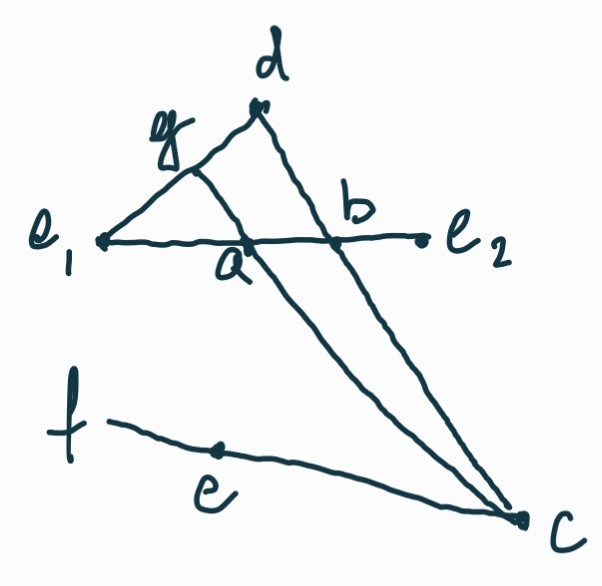
\includegraphics[width=0.5\textwidth]{tempimages/DistinctAndMixture.jpg}
\end{figure}

\begin{proof}
	Let $\ens \distinct \ens[a] = p \ens_1 + \bar{p} \ens_2$ for some $p \in (0, 1)$. Let $\ens[b] = \alpha \ens_1 + \bar{\alpha} \ens_2$ with $0 \leq \alpha < p$. We can do so without loss of generality since switching $\ens_1$ with $\ens_2$ would lead to the case where $1 \geq \alpha > p$. Suppose $\ens[b]$ is not distinct from $\ens$. Then we can find $\ens[c] \in \Ens$ such that $\ens[b] = \beta \ens[c] + \bar{\beta} \ens[d]$ and $\ens = \gamma \ens[c] + \bar{\gamma} \ens[f]$ for some $\ens[d], \ens[f] \in \Ens$ and $\beta, \gamma \in (0, 1)$.
	
	Setting $\epsilon = \frac{p - \alpha}{\bar{\alpha}}$ and $\lambda = \bar{\epsilon} \beta$ we have:
	\begin{align*}
		\ens[a] &= p \ens_1 + \bar{p} \ens_2 = \left(p - \frac{\bar{p}}{\bar{\alpha}} \alpha \right) \ens_1 + \frac{\bar{p}}{\bar{\alpha}} \alpha \ens_1 + \frac{\bar{p}}{\bar{\alpha}} \bar{\alpha}\ens_2 \\
		&= \left(\frac{p\bar{\alpha} - \bar{p}\alpha}{\bar{\alpha}} \right) \ens_1 + \frac{\bar{p}}{\bar{\alpha}} (\alpha \ens_1 + \bar{\alpha} \ens_2) = \left(\frac{p - p\alpha - \alpha + p \alpha}{\bar{\alpha}} \right) \ens_1 + \frac{1 - p + \alpha - \alpha}{\bar{\alpha}} (\alpha \ens_1 + \bar{\alpha} \ens_2) \\
		&= \frac{p - \alpha}{\bar{\alpha}}  \ens_1 + \left( 1 - \frac{p - \alpha}{\bar{\alpha}}\right) (\alpha \ens_1 + \bar{\alpha} \ens_2) = \epsilon \ens_1 + \bar{\epsilon} (\alpha \ens_1 + \bar{\alpha} \ens_2) = \epsilon \ens_1 + \bar{\epsilon} \ens[b] \\
		&= \epsilon \ens_1 + \bar{\epsilon} ( \beta \ens[c] + \bar{\beta} \ens[d] ) = \bar{\epsilon} \beta \ens[c] + \epsilon \ens_1 + \bar{\epsilon} \bar{\beta} \ens[d] = \lambda \ens[c] + \bar{\lambda} \ens[g]
	\end{align*}
	where $\ens[g] = \frac{1}{\bar{\lambda}}\left( \epsilon \ens_1 + \bar{\epsilon} \bar{\beta} \ens[d] \right)$. This means $\ens[a]$ and $\ens$ have a common component, which is a contradiction. Therefore $\ens[b] \distinct \ens$ and $\ens \distinct p \ens_1 + \bar{p} \ens_2$ for all $p \in [0, 1]$
\end{proof}

\begin{prop}
	In a classical ensemble spaces, $\ens \distinct \ens[a]$ and $\ens \distinct \ens[b]$ implies $\ens \distinct p \ens[a] + \bar{p} \ens[b]$ for all $p \in [0,1]$. This is not true in a quantum ensemble space.
\end{prop}

\begin{proof}
	Let $\Ens$ be a classical ensemble space and let $\mu, \nu \in \Ens$ are probability measures on some space $X$. The space of probability measures is a subsets of the space of signed measures. This space can be equipped with an inner product. The space of signed measures with support $U \subseteq X$ form a subspace. This means that, if we can find a $U \subseteq X$ such that both $\mu(U) \neq 0$ and $\nu(U) \neq 0$, we can find a probability measure that is a component of both. That is, two probability measures that have overlapping support have a common component. Conversely, given that convex combination can only expand the support of measures, two probability measure that have no overlapping support have no common components.
	
	Now, suppose $\ens \distinct \ens[a]$ and $\ens \distinct \ens[b]$. This means that the support of $\ens$ is disjoint from the support of both $\ens[a]$ and $\ens[b]$, which will also be disjoint from the support of any mixture of $\ens[a]$ and $\ens[b]$ since the support of the mixture will be the union of the individual supports. This means that $\ens$ will be separate from all mixtures of $\ens[a]$ and $\ens[b]$. The property holds, then, in any classical ensemble space.
	
	Conversely, suppose that $\Ens$ is a quantum ensemble space. Without loss of generality, suppose $\Ens$ is the Bloch sphere and consider the states $x^+$, $x^-$, $z^+$, and $z^-$, which are points on the surface that form a square. These are all separate ensembles. We have $\frac{1}{2} x^+ + \frac{1}{2} x^- = \frac{1}{2} z^+ + \frac{1}{2} z^-$. Therefore a mixture of $x^+$ and $x^-$ has a common component with $z^+$. That is, $z^+ \distinct x^+$ and $z^+ \distinct x^+$ but $z^+ \ndistinct \frac{1}{2} x^+ + \frac{1}{2} x^-$.
\end{proof}

\begin{conj}
	Let $\Ens$ be an ensemble space such that $\ens \distinct \ens[a]$ and $\ens \distinct \ens[b]$ implies $\ens \distinct p \ens[a] + \bar{p} \ens[b]$ for all $p \in [0,1]$. Then it is a classical ensemble space.
\end{conj}


\subsection{Convex hull}

\begin{defn}
	Let $U \subseteq \Ens$ be the subset of an ensemble space. The \textbf{convex hull} of $U$, noted $\hull(U)$ is the set of all possible mixtures that can be constructed with elements contained in $U$.
\end{defn}

\begin{coro}
	The convex hull has the following properties
	\begin{enumerate}
		\item $U \subseteq \hull(U)$
		\item $U \subseteq V \implies \hull(U) \subseteq \hull(V)$
		\item $\hull(\hull(U)) = \hull(U)$
	\end{enumerate}
	and is therefore a closure operation
\end{coro}

\begin{proof}
	1. Every element of $U$ is trivially a mixture of elements of $U$. Therefore $U \subseteq \hull(U)$.
	
	2. Let $\ens \in \hull(U)$. Then it is a mixture of some elements of $U$. Since $U \subseteq V$, then $\ens$ is also the mixture of some elements of $V$ and therefore $\ens \in \hull(V)$.
	
	3. Since mixing is associative and commutative, a mixture of mixtures of $U$ can be reepressed as a mixture of $U$. Therefore for all $\ens \in \hull(\hull(U))$ we have $\ens \in \hull(U)$.
\end{proof}

\begin{conj}
	Let $A \subseteq \Ens$ be a Borel set. Then $\hull(A)$ is also a Borel set.
\end{conj}

\subsection{Fraction and fraction capacity}

\begin{defn}
	Let $\ens, \ens[a] \in \Ens$ be two ensembles. The \textbf{fraction} of $\ens[a]$ in $\ens$ is the greatest mixing coefficient for which $\ens$ can be expressed as a mixture of $\ens[a]$. That is, $\size_{\ens}(\ens[a]) = \sup(\{ p \in [0,1] \, | \, \exists \, \ens_1 \in \Ens \text{ s.t. }  \ens = p \ens[a] + \bar{p} \ens_1 \})$.
\end{defn}

\begin{coro}
	Let $\ens, \ens[a] \in \Ens$, then $\size_{\ens}(\ens[a]) = 0$ if and only if $\ens[a]$ is not a component of $\ens$
\end{coro}

\begin{proof}
	Note that $\ens[a]$ is a component of $\ens$ if we can write $\ens = \lambda \ens[a] + \bar{\lambda} \ens_1$ for some $\lambda \in (0,1]$ and $\ens_1 \in \Ens$. In this case, $\size_{\ens}(\ens[a]) \geq \lambda > 0$. Conversely, if $\size_{\ens}(\ens[a]) > 0$ we can find $\size_{\ens}(\ens[a]) \geq \lambda > 0$ such that $\ens = \lambda \ens[a] + \bar{\lambda} \ens_1$ for some $\ens_1 \in \Ens$.
\end{proof}

\begin{remark}
	We need to take the supremum as the maximum may not exist. For example, consider a discrete classical ensemble space and remove the endpoints. At the moment, there is no reason to rule out such space as unphysical.
\end{remark}

\begin{defn}
	Let $\ens \in \Ens$ be an ensemble and $A \subseteq \Ens$ a Borel set. The \textbf{fraction capacity} of $A$ for $\ens$ is the biggest fraction achievable with convex combinations of $A$. That is, $\fcap_{\ens}(A) = \sup(\size_{\ens}(\hull(A))\cup\{0\})$.
\end{defn}

\begin{coro}
	The fraction capacity uniquely identifies an ensemble. That is, let $\ens_1, \ens_2 \in \Ens$ such that $\ens_1 \neq \ens_2$. Then $\fcap_{\ens_1} \neq \fcap_{\ens_2}$.
\end{coro}

\begin{proof}
	Note that $\ens = 1 \ens_1 + 0 \ens_2$ if and only if $\ens = \ens_1$. Therefore, let $\ens_1, \ens_2 \in \Ens$ such that $\ens_1 \neq \ens_2$. We have $\fcap_{\ens_1}(\{\ens_1\}) = 1$ and $\fcap_{\ens_2}(\{\ens_1\}) \neq 1$. Which means $\fcap_{\ens_1} \neq \fcap_{\ens_2}$
\end{proof}


\begin{prop}
	The fraction capacity for an ensemble is set function that is
	\begin{enumerate}
		\item non negative and unit bounded: $\fcap_{\ens}(A) \in [0,1]$
		\item monotone: $A \subseteq V \implies \fcap_{\ens}(A) \leq \fcap_{\ens}(B)$
		\item subadditive: $\fcap_{\ens}(A \cup B) \leq \fcap_{\ens}(A) + \fcap_{\ens}(B)$
	\end{enumerate}
\end{prop}

\begin{proof}
	1. The fraction capacity takes a subset of $\Ens$ and returns a real value and is therefore a set function. The mixture coefficients are real values between zero and one. The supremum of a set of numbers between zero and one is between zero and one, and therefore the fraction capacity for an ensembles is non negative and unit bounded.
	
	2. The $\hull$ is a monotone function. The inverse image of a set is a monotone function. The supremum is a monotone function. Therefore the fraction capacity is a monotone function.
	
	3. Let $A, B \subseteq \Ens$ and let $p \in [0,1]$ such that $\ens = p \ens_1 + \bar{p} \ens_2$ for some $\ens_1 \in \hull(A \cup B)$ and $\ens_2 \in \Ens$. Since $\ens_1 \in \hull(A \cup B)$, we can write $\ens_1 = \lambda \ens[u] + \bar{\lambda} \ens[v]$ for some $\lambda \in [0,1]$, $\ens[u] \in A$ and $\ens[v] \in B$. Therefore we have $\ens = p \lambda \ens[u] + p \bar{\lambda} \ens[v] + \bar{p} \ens_2$. By the definition of fraction capacity, we must have $p\lambda \leq \fcap_{\ens}(A)$ and $p\bar{\lambda} \leq \fcap_{\ens}(B)$, therefore $p = p\lambda + p\bar{\lambda} \leq \fcap_{\ens}(A) + \fcap_{\ens}(B)$. 	Since $\fcap_{\ens}(A \cup B)$ is the supremum for a set of $p$s for which the expression always holds, we have $\fcap_{\ens}(A \cup B) \leq \fcap_{\ens}(A) + \fcap_{\ens}(B)$. The probability measure is subadditive.
\end{proof}

\subsection{Vector space embedding}

\begin{defn}
	 Let $\ens[\rho] = p \ens_1 + \bar{p} \ens_2$ with $p \in (0,1)$. Then we say that $\ens_2$ is a $p$-\textbf{complement} of $\ens_1$ towards $\ens[\rho]$. An ensemble space is \textbf{complemented} if all $p$-complements are unique for all $p \in (0, 1)$.
\end{defn}

\begin{prop}\label{pm_es_complementedIsVectorSpace}
	An ensemble space is complemented if and only if it is a convex subset of a real vector space for which mixtures are linear combination.
\end{prop}

\begin{proof}
	Theorem 4 in \url{https://arxiv.org/abs/1105.1270} states that a convex space embeds into a real vector space with $c_\lambda(x,y) = \lambda x + \bar{\lambda}y$ if and only if
	$$ c_\lambda(x,y) = c_\lambda(x,z) \; \forall \lambda \in (0,1) \implies y = z.$$ This property, called cancellative property, is exactly the condition that the $\lambda$-complement is unique.
\end{proof}

\begin{prop}
	Discrete classical ensemble spaces, continuous classical ensemble spaces and quantum ensemble spaces satisfy the axiom of mixture and are complemented ensemble spaces.
\end{prop}

\begin{proof}
	The space of probability measures, discrete or continuous, $\Ens$ is a convex subset of the vector space of finite signed measures. This means that it is closed under convex combinations: $\sum p_i \ens_i$ for all $\{e_i\} \subseteq \Ens$ and $\sum p_i = 1$. The properties of mixing are inherited from the properties of linear combinations. Therefore the discrete and continuous classical ensemble spaces satisfy the axiom of mixture. Moreover, $\Ens$ is a convex subset of a vector space, it is complemented by proposition \ref{pm_es_complementedIsVectorSpace}.
	
	Similarly, the space of positive semi-definite self-adjoint operators with trace one is a convex subset of the vector space of self-adjoint operators. Therefore it is closed under convex combinations and it will satisfy the axiom of mixture. Moreover, it is complemented convex by proposition \ref{pm_es_complementedIsVectorSpace}.
\end{proof}


\begin{remark}
	Since all current physical ensemble spaces are complemented, it is not yet clear whether an ensemble space must be complemented or not. It is difficult to justify as it is a claim on existence of more refined ensembles. It may very well be that this is just an assumption on the decomposition, which may fail in new physical conditions (e.g. at Planck scale). It may also be something that the strict concavity of the entropy requires.
\end{remark}

\begin{remark}
	Assuming that the mixing operation is continuous does not guarantee that we can vector space that embeds the convex space is a topological vector space. See \url{https://math.stackexchange.com/questions/4921905/cancellative-convex-spaces-and-topological-vector-spaces}. The issue is we have no guarantee of continuity on the inverse (i.e. subtraction, multiplication for a negative number).
\end{remark}

\section{Quantities}

In the same way that we define ensembles first, we define quantities through their expectation over ensembles. The possible value for pure states will need to be recovered with constructions that are connected to spectral theory.

\begin{defn}
	A \textbf{statistical variable}, or simply variable, is a numerical quantity that is well-defined over all ensembles. Formally, it is a continuous linear real valued operator on $\Ens$. That is, $F : \Ens \to \mathbb{R}$ such that $F(p \ens_1 + \bar{p} \ens_2) = p F(\ens_1) + \bar{p} F(\ens_2)$. 
\end{defn}

\begin{justification}
	Continuity is required since the value of a variables is experimentally verifiable. The linearity of the operator associated to the quantity stems for the expectation. When mixing two different processes, the measured value will only depend on the selection at that particular time, and therefore each process will contribute to the final value based on its fraction.
	
	Note that the value cannot be infinite. The only way to measure infinity is if the measured average keeps increasing in time. This would be a contradiction on the assumption that the ensemble is at equilibrium.
\end{justification}

\begin{remark}
	Note that variables will have a contiguous range on the ensembles because, given two ensembles with different values, we can mix them to obtain any intermediate value. This does not mean that the variable can take all possible values on pure states. For example, the number of particles in a pure state will necessarily be a non-negative integer, but we can mix those to create ensembles that have non-integer average number of particles.
\end{remark}

\begin{prop}
	Let $\Ens$ be a complemented ensemble space. Then a statistical variable $F$ induces a semi-norm on the vector space that embeds $\Ens$.
\end{prop}

\begin{proof}
	Let $F$ be a variable on $\Ens$ and let $V$ be the vector space that embeds $\Ens$. Extend $F$ on $V$ such that $F(a\ens) = |a| F(\ens)$. Then, according to the definition given after 1.1 in \url{https://personal.math.ubc.ca/~cass/research/pdf/TVS.pdf} $F$ is a semi-norm.
\end{proof}

\begin{defn}
	A \textbf{quantifiable} ensemble space is an ensemble space where each ensemble can be identified by a set of statistical variables. That is, there is family of statistical variables $F_i : \Ens \to \mathbb{R}$ such that, given $\ens_1, \ens_2 \in \Ens$, $F_i(\ens_1) = F_i(\ens_2)$ for all $i$ if and only if $\ens_1 = \ens_2$. Moreover, the topology is generated by those variables.
\end{defn}

\begin{prop}
	A quantifiable complemented ensemble space is embedded into a Hausdorff locally compact topological vector space.
\end{prop}

\begin{proof}
	The ensemble is complemented, therefore it is embedded into a vector space. The topology of the ensemble space is generated by the statistical variables, which induce semi-norms on the vector space. This means that the topology of the vector space is generated by a countable set of semi-norms, and is therefore a locally convex topological vector space. See Prop 2.2 in \url{https://personal.math.ubc.ca/~cass/research/pdf/TVS.pdf}.
	
	The statistical variables fully identify each ensemble, which means that, if two elements are different, one semi-norm will give a non-zero value for the distance function associated with it. This means that the topology is Hausdorff. See Prop 2.6 in \url{https://personal.math.ubc.ca/~cass/research/pdf/TVS.pdf}.
\end{proof}

\begin{coro}
	A quantifiable ensemble spaces is fully determined by countably many statistical variables.
\end{coro}

\begin{proof}
	The topology of an ensemble space is second countable. A Hausdorff second countable locally compact topological vector space can always be generated by countably many semi-norms.
\end{proof}

\begin{remark}
	Note that we are missing completeness in terms of the semi-norms to obtain a Fr\'echet space. It is not clear whether this is required since, for example, $L^1(\mathbb{R}^{2n}) \cap C(\mathbb{R}^{2n})$ is not Fr\'echet.
\end{remark}

\begin{conj}
	Discrete/continuous classical ensemble spaces and quantum ensemble spaces are quantifiable.
\end{conj}

\begin{proof}
	For discrete classical spaces, the expectation of the indicator of each extreme point defines a countable set of quantities that fully identifies the distribution.
	
	For continuous classical spaces, $L^1(\mathbb{R}^{2n}) \cap C(\mathbb{R}^{2n})$ is a Hausdorff locally convex topological spaces.
	
	TODO Quantum (note that we are looking at the space of density operators with finite expectation value for position and momentum).
\end{proof}

\begin{conj}
	Quantifiable spaces are complemented.
\end{conj}

\begin{remark}
	Not clear whether this is true. The idea is that one can create open balls with quantities, which are, in a sense, symmetric neighborhoods. These may define unique inverses.
\end{remark}

\begin{conj}
	If all ensembles can be connected by linear transformations parameterized by real quantities, then the ensemble is quantifiable.
\end{conj}

\begin{remark}
	Note clear whether this is true. The idea is that the time interval can be used to define variables. A more sophisticated conjecture may look at the space of generators of Lie groups. This would link the topology of time to the topology of the ensemble space. If the topology of time is not that of the real numbers, then, the ensemble space must change significantly.
\end{remark}

% TODO: for later
%\begin{conj}
%	Let $\ens \in \Ens$ and $A \subset \Ens$. Let $\{\ens[a]_i\}$ and $\{\ens[b]_i\}$ be two maximal increasing $A$-component sequence. Then $\lim\limits_{i \to \infty} F(\ens[a]_i) = \lim\limits_{i \to \infty} F(\ens[a]_i)$ for any quantities $F$.
%\end{conj}

\begin{proof}
	Check that the all maximal sequences give the same value.
\end{proof}

\section{Entropy}

The third and final property of ensembles is that they have a well-defined entropy, that corresponds to the thermodynamic entropy. That is, while in information theory one can define all sorts of measure of uncertainty/information/variability, there is one that corresponds to a physically measurable quantity.

\begin{defn}
	Given the coefficients $\{p_i\} \in [0,1]$ such that $\sum p_i = 1$, the \textbf{entropy of the coefficients} (also known as Shannon entropy) is defined as $I(\{p_i\}) = - \sum p_i \log p_i $.
\end{defn}

\begin{axiom}[Axiom of entropy]
	An ensemble space $\Ens$ is equipped a function $S : \Ens \to \mathbb{R}$ called \textbf{entropy} with the following properties
	\begin{itemize}
		\item \textbf{Continuity}
		\item \textbf{Strict concavity}: $S(p_1\ens_1 + p_2 \ens_2) \geq p_1 S(\ens_1) + p_2 S(\ens_2)$ with the equality holding if and only if $\ens_1 = \ens_2$
		\item \textbf{Upper variability bound}: $S(p_1\ens_1 + p_2 \ens_2) \leq I(p_1, p_2) + p_1 S(\ens_1) + p_2 S(\ens_2)$; if the equality hold then, $e_1$ and $e_2$ are \textbf{non-overlapping} or \textbf{orthogonal}, noted $e_1 \disjunct e_2$
	\end{itemize}
\end{axiom}

\begin{justification}
	The entropy quantifies the variability of the elements within the ensemble. This justifies the existence of the entropy.
	
	Small changes in the ensemble should produce small changes in the variability, which justifies continuity. Mixing different ensembles will increase the variability, which justifies concavity. Mixing the same ensemble, however, should not increase the variability, which justifies strict concavity. 
	
	The variability increase is maximal when the two ensembles are non-overlapping, meaning they have no elements in common. In this case, the increase in variability is given only by the coefficients and must follow the Shannon entropy as it is the only continuous indicator of variability that is linear in probability. This justifies the upper bound.
\end{justification}

\begin{conj}
	The entropy can be derived to be continuous, instead of imposing it.
\end{conj}

\begin{remark}
	We have found proofs that convex/concave quantities on a convex subspace of $\mathbb{R}^n$ are continuous. The proof may be generalizable to any topological convex space.
\end{remark}

\begin{conj}
	The upper bound of the entropy can be uniquely determined, instead of imposing it.
\end{conj}

\begin{remark}
	In \url{https://arxiv.org/abs/1912.02012} we showed how the Shannon entropy quantifies the variability of elements within a distribution. Is it possible to rederive $I$ from requirements on convex spaces instead of distributions in particular? This would make the axiom less ad-hoc.
	
	The difference is that in that proof we are automatically assuming that things can be decomposed into orthogonal elements, and that mixture of orthogonal elements remain orthogonal (i.e. the axiom of entropic orthogonality). This should imply that mixture of many orthogonal element saturate the upper bound. Once that is assumed, then one can find the entropy difference for a generic uniform distribution, then for a rational distribution and then, by continuity, for all reals.
\end{remark}

\begin{conj}\label{pm_es_ensemblesAreTVS}
	An ensemble space embeds in a topological vector space if and only if it is complemented (i.e. cancellative).
\end{conj}

\begin{proof}
	The idea is to use the entropy to show that open balls are part of the topology, and then use this to show that multiplication for a scalar is continuous. The continuity of addition should come from the continuity of the mixing operation.
\end{proof}

\begin{axiom}[Axiom of entropic orthogonality]
	The entropy function of an ensemble space obeys the following properties
	\begin{itemize}
		\item \textbf{Orthogonality implies separateness}: $\ens_1 \disjunct \ens_2$ implies $\ens_1 \distinct \ens_2$
		\item \textbf{Mixtures preserve orthogonality}: let $\ens_1 = p \ens_2 + \bar{p} \ens_3$, then $\ens_4 \disjunct \ens_1$ if and only if $\ens_4 \disjunct \ens_2$ and $\ens_4 \disjunct \ens_3$
	\end{itemize}
\end{axiom}

\begin{justification}
	If two ensembles are disjunct, they have no elements in common. Therefore there will be no common component with the two. We are justified to assume that disjunctness implies distinctness.
	
	Suppose an ensemble $\ens_1$ is disjunct from the mixture of two ensembles $\ens_2$ and $\ens_3$. That it has no elements in common with the mixture, which means it has no elements in common with either of them. Therefore $\ens_1$ is disjunct from both $\ens_2$ and $\ens_3$. Now suppose $\ens_1$ is disjunct from both $\ens_2$ and $\ens_3$. That it means it has no elements in common with either of them, and therefore it does not have any elements in common with their mixture. Therefore $\ens_1$ is disjunct from the mixture of two ensembles $\ens_2$ and $\ens_3$. We are justified to assume that mixtures preserve disjunctness.
\end{justification}

\begin{remark}
	It is unclear whether ``orthogonality implies separatenes'' is an independent axiom. It is possible to prove that two orthogonal ensembles are not one the component of the other. The entropy of the coefficients (i.e. the Shannon entropy) has a vertical asymptote at each end. If two elements are orthogonal, the entropy along the segment that connects the two follows that function plus a linear function, which does not change the vertical asymptotes. Therefore the segment cannot be extended while preserving the convexity of the entropy, and therefore the two orthogonal elements must the extremes of the line that connects the two. This is necessary for separateness, but it is not sufficient.
\end{remark}

\begin{remark}
	It may be possible to show that mixtures preserve orthogonality is an independent axiom. Take the 2 dimensional simplex (i.e. a triangle) that represent a classical discrete probability space over three elements. Take the standard entropy, which will satisfy ``mixtures preserve orthogonality''. This is because the middle point has entropy $\log 3$. We can imagine changing the entropy so that it is a little bit lower in the center but it is unchanged on the sides. If that is possible, then the new entropy may still satisfy all other axioms.
\end{remark}

\begin{prop}
	The discrete classical ensemble spaces, continuous classical ensemble spaces and quantum ensemble spaces satisfies the axiom of mixture and the axiom of entropic disjunctness.
\end{prop}

\begin{proof}
	In both classical cases, the entropy is a function of only the probabilities of the decomposition in terms of pure states. The function is continuous in terms of those variables as $x \log x$ is a continuous function. [TODO find short proof of convexity and maximum bound]
	
	In the quantum case, the entropy is a continuous function of the density operator as the trace, multiplication and logarithm of an operator are all continuous functions. [TODO find short proof of convexity and maximum bound]
\end{proof}

\begin{remark}
	There should be an interplay between convexity and entropy which limits either the space or the possible entropy. For example, consider a line. It is a convex space with no extreme points. We can parameterize the space with a variable $x$ such that the mixture of two ensembles is identified by the average $x$. Entropy can be written as $S(x)$. Since $S(x)$ is strictly concave over an infinite range, it will tend to minus infinity either when $x$ tends to infinity or minus infinity. Now take a line that intersects the curve. This will intersect it at only two points. By strict convexity, there is only going to be a single point with maximum vertical distance to the line, which has to be greater than zero. Now imagine moving the line down by one vertical unit. The vertical distance now is greater than one. This means that the average entropy can increase more than one during mixture, which violates the upper variability bound. Therefore a line cannot be an ensemble space.
	
	Note that an open segment is absolutely fine. We can, in fact, imagine a two state discrete classical ensemble space with the endpoint removed. This suggests that the convex space knows something about the geometry (probably parallelism and ratio of length - i.e. the affine structure).
\end{remark}

\begin{conj}
	Let $\ens_1, \ens_2 \in \Ens$ be such that $p\ens + \bar{p} \ens_1 = p\ens + \bar{p} \ens_2$ for some $p \in (0, 1)$ and $\ens \in \Ens$. Then $\ens_1$ and $\ens_2$ are not disjunct.
\end{conj}

\begin{remark}
	It seems very unlikely that differences in states that can be obscured by mixing would correspond to disjunct states. The more general question is whether the strict concavity of the entropy allows non-complemented spaces.
\end{remark}

\begin{defn}
	Two sets of ensembles $U, V \subseteq \Ens$ are orthogonal if $\ens_1 \disjunct \ens_2$ for all $\ens_1 \in U$ and $\ens_2 \in V$. 
\end{defn}

\subsection{Reducible ensemble spaces}

\begin{defn}
	An ensemble space $\Ens$ is \textbf{reducible} if separate ensembles are also orthogonal. That is, $\ens_1 \distinct \ens_2$ implies $\ens_1 \disjunct \ens_2$.
\end{defn}

\begin{justification}
	Given that $\ens_1 \disjunct \ens_2$ implies $\ens_1 \distinct \ens_2$, classical spaces add the opposite implication. Therefore they exclude the case where two ensembles are disjunct but not distinct. This case describes two ensembles that have elements in common, but there is no ensemble corresponding to those common elements. That is, we cannot refine the ensembles into three distinct ones: one with only elements of the first, one with only elements of the second and one with elements of both. In other words, we cannot reduce the coarser description of the system into finer distinct descriptions. In the excluded case, then, the coarser description is irreducible into finer ensembles. This justifies the definition.
	
	As we prove below, that case does not exist in classical mechanics, but exists in quantum mechanics. This justifies calling the property classical.
\end{justification}

\begin{prop}
	Continuous and discrete classical ensemble spaces are reducible.
\end{prop}

\begin{proof}
	In both cases, ensembles are probability measures: the first over the Borel algebra of a symplectic manifold; the second over the power set of countably many elements. In both cases, the upper bound of the entropy is maximized if and only if the probability measures being combined have disjoint support. This means that two ensembles are disjunct if and only if the respective probability measures have disjoint support. Intuitively, two probability distributions can have a common sub-distribution if and only if they overlap. Therefore two ensembles representing probability measures with disjoint support are exactly ensembles that are distinct. Therefore, in both cases, the ensemble space is reducible.
\end{proof}

\begin{conj}
	An ensembles space is reducible only if it is classical.
\end{conj}

\begin{remark}
	The reverse direction cannot, in general, work. Take the subspace of a finite classical discrete ensemble space such the maximum probability of any element is $k < 1$. This corresponds to a simplex of the same dimension, with the same center, but scaled in the interior. Given that it is a convex subset of an ensemble space, it will satisfy all the axioms, except it will contain no orthogonal ensembles. Yet, it contains separate ensembles, which cannot be orthogonal.
\end{remark}

\begin{remark}
	The above property should ultimately be responsible for the single decomposition in terms of pure states.
\end{remark}

\begin{prop}
	Continuous and discrete classical ensemble spaces are reducible.
\end{prop}

\begin{proof}
	In both cases, ensembles are probability measures: the first over the Borel algebra of a symplectic manifold; the second over the power set of countably many elements. In both cases, the upper bound of the entropy is maximized if and only if the probability measures being combined have disjoint support. This means that two ensembles are disjunct if and only if the respective probability measures have disjoint support. Intuitively, two probability distributions can have a common sub-distribution if and only if they overlap. Therefore two ensembles representing probability measures with disjoint support are exactly ensembles that are distinct. Therefore, in both cases, the ensemble space is reducible.
\end{proof}

\section{Effective count}

\begin{prop}[Exponential entropy subadditivity]\label{pm_es_exponentialEntropySubadditivity}
	Let $\ens_1, \ens_2 \in \Ens$. Let $S_1 = S(\ens_1)$ and $S_2 = S(\ens_2)$. Let $\ens = p \ens_1 + \bar{p} \ens_2$ for some $p \in [0,1]$ and $S = S(\ens)$. Then $2^S \leq 2^{S_1} + 2^{S_2}$, with the equality if and only if $\ens_1$ and $\ens_2$ are disjunct and $p = \frac{2^{S_1}}{2^{S_1} + 2^{S_2}}$.
\end{prop}

\begin{proof}
	If $p$ is fixed, the upper variability bound of entropy is saturated only if $\ens_1$ and $\ens_2$ are disjunct by definition. The entropy maximum for the mixed ensemble can only be achieved when the elements are disjunct, for some value of $p$.
	
	Now fix $S_1$ and $S_2$. The entropy of the mixture depends only on $p$, so we need to find the $p$ that maximizes the expression. Since $\ens_1$ and $\ens_2$ are disjunct, $S(p \ens_1 + \bar{p}\ens_2) =  - p \log p - \bar{p} \log \bar{p} + p S_1 + \bar{p} S_2$ which is a smooth function of $p$.
	\begin{equation}
		\begin{aligned}
			0 = \frac{dS}{dp} &= \frac{d}{dp} S(\ens) =\frac{d}{dp} \left( - p \log p - \bar{p} \log \bar{p} + p S_1 + \bar{p} S_2 \right) \\
			&= - \log p - 1 + \log \bar{p} + 1 + S_1 - S_2 \\
			\log \frac{p}{\bar{p}} &= \log 2^{S_1} - \log 2^{S_2} \\
			\log \frac{p}{1-p} &= \log \frac{2^{S_1}}{2^{S_2}}  \\
			p 2^{S_2} &= (1-p) 2^{S_1}  \\
			p (2^{S_1} + 2^{S_2}) &= 2^{S_1}  \\
			p &= \frac{2^{S_1}}{2^{S_1} + 2^{S_2}}  \\
		\end{aligned}
	\end{equation}
	Having found the value of $p$ that maximizes the entropy, we can calculate the maximum entropy.
	\begin{equation}
	\begin{aligned}
		\bar{p} &= 1- \frac{2^{S_1}}{2^{S_1} + 2^{S_2}} = \frac{2^{S_2}}{2^{S_1} + 2^{S_2}} \\
		S &= S(\ens) = - p \log p - \bar{p} \log \bar{p} + p S_1 + \bar{p} S_2  \\
		&= - \frac{2^{S_1}}{2^{S_1} + 2^{S_2}} \log \frac{2^{S_1}}{2^{S_1} + 2^{S_2}} - \frac{2^{S_2}}{2^{S_1} + 2^{S_2}} \log \frac{2^{S_2}}{2^{S_1} + 2^{S_2}} \\
		&+ \frac{2^{S_1}}{2^{S_1} + 2^{S_2}} \log 2^{S_1} + \frac{2^{S_2}}{2^{S_1} + 2^{S_2}} \log 2^{S_2} \\
		&= \frac{2^{S_1}}{2^{S_1} + 2^{S_2}} \log \left( 2^{S_1} + 2^{S_2} \right) + \frac{2^{S_2}}{2^{S_1} + 2^{S_2}} \log \left( 2^{S_1} + 2^{S_2} \right) \\
		&= \frac{2^{S_1} + 2^{S_2}}{2^{S_1} + 2^{S_2}} \log \left( 2^{S_1} + 2^{S_2} \right) \\
		\log 2^S &= \log \left( 2^{S_1} + 2^{S_2} \right) \\
		2^S &=  2^{S_1} + 2^{S_2}  \\
	\end{aligned}
	\end{equation}
	Therefore the maximum entropy obtainable through a mixture is $S = \log (2^{S_1} + 2^{S_2})$ which is obtained when $\ens_1$ and $\ens_2$ are disjunct and $p = \frac{2^{S_1}}{2^{S_1} + 2^{S_2}}$.
\end{proof}

\begin{defn}
	Let $U \subseteq \Ens$ be the subset of an ensemble space. The \textbf{effective count} of $U$ is defined as $\size(U) = \sup(2^{S(\hull(U))})$ if $U \neq \emptyset$ and $\size(U) = 0$ otherwise.
\end{defn}

\begin{prop}
	The effective count is a set function that is
	\begin{enumerate}
		\item non negative: $\size(U) \in [0, +\infty]$
		\item monotone: $U \subseteq V \implies \size(U) \leq \size(V)$
		\item subadditive: $\size(U \cup V) \leq \size(U) + \size(V)$
		\item additive over disjunct sets: $U \disjunct V \implies \size(U \cup V) = \size(U) + \size(V)$ 
	\end{enumerate}
\end{prop}

\begin{proof}
	1. The effective count takes a subset of $\Ens$ and returns a real value and is therefore a set function. The exponential can only return non-negative values, therefore the effective count of a set is non-negative. 
	
	2. Let $U, V \subseteq \Ens$ such that $U \subseteq V$. If $U = \emptyset$, we have $\size(U) = 0$. Since $\size(V)$ is non-negative, $\size(U) \leq \size(V)$. If $U \neq \emptyset$, $\hull(U) \subseteq \hull(V)$ and therefore $2^{S(\hull(U))} \subseteq 2^{S(\hull(V))}$. This means that the supremum of the first set cannot be greater than the supremum of the second set, and therefore $\size(U) \leq \size(V)$. The effective count is a monotone set function.
	
	3. Let $U, V \subseteq \Ens$ and let $\ens \in \hull(U \cup V)$. Then we can write $\ens = p \ens[u] + \bar{p} \ens[v]$ for some $p \in [0,1]$, $\ens[u] \in U$ and $\ens[v] \in V$. By \ref{pm_es_exponentialEntropySubadditivity} and the definition of effective count, $2^{S(\ens)} = 2^{S(\ens[u])} + 2^{S(\ens[v])} \leq \size(U) + \size(V)$. Since this is true for any element of $\hull(U \cup V)$, the supremum of the exponential entropy cannot exceed the sum of the effective counts. Therefore $\size(U \cup V) \leq \size(U) + \size(V)$, the effective count is subadditive.
	
	4. Let $U, V \subseteq \Ens$ be two disjunct subsets. Let $\{\ens[u]_i\} \subset U$ be a sequence of ensembles such that $2^{S(\ens[u]_i)} \to \size(U)$ and let $\{\ens[v]_i\} \subset V$ be a sequence of ensembles such that $2^{S(\ens[v]_i)} \to \size(V)$. Consider $\ens_i = p_i \ens[u]_i + \bar{p_i} \ens[v]_i$ where $p_i = \frac{2^{S(\ens[u]_i)}}{2^{S(\ens[u]_i)} + 2^{S(\ens[v]_i)}}$. Then, by \ref{pm_es_exponentialEntropySubadditivity}, $2^{S(\ens_i)} = 2^{S(\ens[u]_i)} + 2^{S(\ens[v]_i)}$. This means that $2^{S(\ens_i)} \to \size(U) + \size(V)$. Therefore $\size(U \cup V) \geq \size(U) + \size(V)$. Combining with the previous result, $\size(U \cup V) = \size(U) + \size(V)$. Therefore effective count, as set function, is additive over disjunct sets of ensembles.
\end{proof}

\section{Entropic geometry}

We now show that entropy imposes a geometric structure on the ensemble space.

\begin{defn}
	Given two ensembles $\ens_1, \ens_2 \in \Ens$, the \textbf{mixing entropy}, also called Jensen-Shannon divergence, is the increase in entropy associated to their mixture. That is:
	$$MS(\ens_1, \ens_2) = S\left(\frac{1}{2}\ens_1 + \frac{1}{2} \ens_2\right) - \left(\frac{1}{2} S(\ens_1) + \frac{1}{2} S(\ens_2)\right).$$
\end{defn}

\begin{coro}
	The mixing entropy obeys the following bounds
	$$ 0 \leq MS(\ens_1, \ens_2) \leq 1.$$
	The lower bound is satisfied if and only if $\ens_1 = \ens_2$ and the upper bound is satisfied if and only if $\ens_1 \disjunct \ens_2$.
\end{coro}

\begin{proof}
	The bounds descend directly from the bounds on entropy. By strict concavity, $S(p_1\ens_1 + p_2 \ens_2) \geq p_1 S(\ens_1) + p_2 S(\ens_2)$, which means $S(p_1\ens_1 + p_2 \ens_2) - p_1 S(\ens_1) - p_2 S(\ens_2) \geq 0$, and in particular $S(\frac{1}{2} \ens_1 + \frac{1}{2} \ens_2) - \frac{1}{2} S(\ens_1) - \frac{1}{2} S(\ens_2) = MS(\ens_1, \ens_2) \geq 0$. By strict concavity, the equality holds if and only if $\ens_1 = \ens_2$
	
	By the upper variability bound, $S(p_1\ens_1 + p_2 \ens_2) \leq I(p_1, p_2) + p_1 S(\ens_1) + p_2 S(\ens_2)$, which means $S(p_1\ens_1 + p_2 \ens_2) - p_1 S(\ens_1) - p_2 S(\ens_2) \leq I(p_1, p_2)$, and in particular $S(\frac{1}{2} \ens_1 + \frac{1}{2} \ens_2) - \frac{1}{2} S(\ens_1) - \frac{1}{2} S(\ens_2) = MS(\ens_1, \ens_2) \leq I(\frac{1}{2}, \frac{1}{2}) = 1$. Given that $\ens_1$ and $\ens_2$ are disjunct by definition if they saturate the upper variability bound, the equality holds if and only if $\ens_1$ and $\ens_2$ are disjunct.
\end{proof}

\begin{prop}
	In discrete and continuous classical cases, the mixing entropy coincides with the Jensen-Shannon divergence. In quantum spaces it coincindes with the quantum Jensen-Shannon divergence.
\end{prop}

\begin{proof}
	Looking at the definitions \href{https://en.wikipedia.org/wiki/Jensen%E2%80%93Shannon_divergence}{Jensen-Shannon divergence}, one can see that
	$$ JSD(\ens_1, \ens_2) = S\left(\frac{1}{2}\ens_1 + \frac{1}{2}\ens_2 \right)  - \frac{1}{2} \left(S(\ens_1) + S(e_2)\right) = MS(\ens_1, \ens_2)$$.
	The same is true for the quantum case:
	$$ QJSD(\ens_1, \ens_2) = S\left(\frac{1}{2}\ens_1 + \frac{1}{2}\ens_2 \right)  - \frac{1}{2} \left(S(\ens_1) + S(\ens_2)\right) = MS(\ens_1, \ens_2)$$.
\end{proof}

\begin{defn}
	An ensemble space is \textbf{geometric} if it is complemented and has a twice differentiable entropy with respect to the mixing coefficients.
\end{defn}

\begin{conj}
	A geometric ensemble space is a convex subset of a real vector space. Moreover, every finite dimensional subspace is a smooth manifold.
\end{conj}

\begin{proof}
	Since a geometric ensemble space is complemented, it embeds into a real vector space. If conjecture \ref{pm_es_ensemblesAreTVS} holds, then it is a topological vector space. Every finite dimensional subspace $V$, then, is locally $R^n$ with a topology. This would be enough to claim $V$ is a manifold. The differentiable structure is imposed by requiring coordinates that coordinates are twice differentiable with respect to the mixing coefficients.
\end{proof}

\begin{remark}
	The above restriction is useful to recover standard elements of differential geometry. It is an open question to understand whether other conditions already imply these requirements, or whether a more general setting can be developed. For example, in a classical space every ensemble can be understood as the mixture of orthogonal elements. Therefore the entropy can be proven the Shannon/Gibbs entropy, and therefore it is infinitely smooth with respect to the coefficients. A classical space, then, would be automatically geometric. Similar arguments may exist for a quantum space. Additionally, it may be that the convex structure may be enough to define a generalized version of tangent space.
\end{remark}

\begin{defn}
	Let $V \subseteq \Ens$ be a differentiable manifold embedded in the ensemble space. Let $\ens \in \Ens$ be an ensemble and $T_{\ens}$ the tangent space at that point. The \textbf{norm} of $\delta \ens \in T_{\ens}$ is given by
	$$ \lVert \delta \ens \rVert_{\ens} = \sqrt{ 8 MS(\ens, \ens + \delta \ens) }.$$
	The \textbf{metric tensor} (i.e. the inner product between $\delta \ens_1 , \delta \ens_2 \in T_{\ens}$ ) is given by
	$$ g_{\ens}( \delta \ens_1, \delta \ens_2 ) = \frac{1}{2} \left( \lVert \delta \ens_1 + \delta \ens_2 \rVert_{\ens}^2 - \lVert \delta \ens_1 \rVert_{\ens}^2 - \lVert \delta \ens_2 \rVert_{\ens}^2 \right).$$
\end{defn}

\begin{thrm}
	Let $\Ens$ be a geometric ensemble space and $V \subseteq \Ens$ a differentiable manifold embedded in the ensemble space. Then
	$$ \lVert \delta \ens \rVert_{\ens}^2 = - \frac{\partial^2 S}{\partial \ens^2}(\delta \ens , \delta \ens) $$
	and 
	$$ g_{\ens}( \delta \ens_1, \delta \ens_2 ) = - \frac{\partial^2 S}{\partial \ens ^2}( \delta \ens_1, \delta \ens_2 ).$$
	Then $V$ is a Riemannian manifold with $g_{\ens}$ as the metric tensor and $\lVert \cdot \rVert_{\ens}$ as the norm.
\end{thrm}

\begin{proof}
	To recover the first two expression, we simply have to calculate the leading term. Since the entropy is twice differentiable, we can expand it as
\begin{equation}
	\begin{aligned}
		S(\ens + \delta \ens) &= S(\ens) + \frac{\partial S}{\partial \ens} \delta \ens + \frac{1}{2} \frac{\partial^2 S}{\partial \ens^2} \delta \ens \delta \ens + O(\delta \ens ^3).
	\end{aligned}
\end{equation}
Expanding the definition of $MS$, we have
\begin{equation}
	\begin{aligned}
		MS(\ens, \ens + \delta \ens) &= S\left(\frac{1}{2} \ens + \frac{1}{2}(\ens + \delta \ens) \right) - \frac{1}{2} S(\ens) - \frac{1}{2} S(\ens+\delta \ens) \\
		&=  S\left(\ens + \frac{1}{2} \delta \ens \right) - \frac{1}{2} S(\ens) - \frac{1}{2} S(\ens+\delta \ens) \\
		&= S(\ens) + \frac{\partial S}{\partial \ens} \frac{1}{2}\delta \ens + \frac{1}{2} \frac{\partial^2 S}{\partial \ens^2} \frac{1}{2}\delta \ens \frac{1}{2}\delta \ens + O(\delta \ens ^3) \\
		&- \frac{1}{2} S(\ens) - \frac{1}{2} \left( S(\ens) + \frac{\partial S}{\partial \ens} \delta \ens + \frac{1}{2} \frac{\partial^2 S}{\partial \ens^2} \delta \ens \delta \ens + O(\delta \ens ^3) \right) \\
		&= S(\ens) + \frac{1}{2} \frac{\partial S}{\partial \ens} \delta \ens + \frac{1}{8} \frac{\partial^2 S}{\partial \ens^2} \delta \ens \delta \ens \\
		&- S(\ens) - \frac{1}{2} \frac{\partial S}{\partial \ens} \delta \ens - \frac{1}{4} \frac{\partial^2 S}{\partial \ens^2} + O(\delta \ens ^3) \\
		&= - \frac{1}{8} \frac{\partial^2 S}{\partial \ens^2} \delta \ens \delta \ens + O(\delta \ens ^3).
	\end{aligned}
\end{equation}

Therefore
$$ \lVert \delta \ens \rVert^2 = 8 MS(\ens, \ens + \delta \ens) = -  \frac{\partial^2 S}{\partial \ens^2} (\delta \ens, \delta \ens).$$

We can now substitute the norm to the definition of metric tensor. We have
\begin{equation}
	\begin{aligned}
		g_{\ens}(\delta \ens_1, \delta \ens_2 ) &= \frac{1}{2} \left( \lVert \delta \ens_1 + \delta \ens_2 \rVert^2 - \lVert \delta \ens_1 \rVert^2 - \lVert \delta \ens_2 \rVert^2 \right) \\
		&= \frac{1}{2} \left( - \frac{\partial^2 S}{\partial \ens^2} (\delta \ens_1 + \delta \ens_2, \delta \ens_1 + \delta \ens_2) + \frac{\partial^2 S}{\partial \ens^2} (\delta \ens_1, \delta \ens_1) + \frac{\partial^2 S}{\partial \ens^2} (\delta \ens_2, \delta \ens_2) \right) \\
		&= - \frac{1}{2} \left(  \frac{\partial^2 S}{\partial \ens^2} (\delta \ens_1, \delta \ens_1) + \frac{\partial^2 S}{\partial \ens^2} (\delta \ens_1, \delta \ens_2) + \frac{\partial^2 S}{\partial \ens^2} (\delta \ens_2, \delta \ens_1) + \frac{\partial^2 S}{\partial \ens^2} (\delta \ens_2, \delta \ens_2) \right. \\
		&-  \left. \frac{\partial^2 S}{\partial \ens^2} (\delta \ens_1, \delta \ens_1) - \frac{\partial^2 S}{\partial \ens^2} (\delta \ens_2, \delta \ens_2) \right) \\
		&= - \frac{\partial^2 S}{\partial \ens^2} (\delta \ens_1, \delta \ens_2) \\
	\end{aligned}
\end{equation}

	Let us now take an embedded manifold $V \subseteq \Ens$. It will have a smooth structure inherited from the ensemble space.
	
	Let us now show that $g$ is a metric tensor. Restricted to $V$, $g|_V$ is the Hessian of the entropy $S$. Therefore it is a symmetric rank two tensor which means a symmetric bilinear function of the arguments. Since the entropy is strictly concave, the Hessian is negative definite and therefore $g$ is positive definite. Therefore $(V, g|_V)$ is a Riemannian manifold.
\end{proof}

\begin{prop}
	For a classical ensemble space, the metric corresponds to the Fisher-Rao metric.
\end{prop}

\begin{proof}
	Recall that, given a manifold of probability distributions over $X$ parametrized by $\theta^i$, the \href{https://en.wikipedia.org/wiki/Fisher_information_metric}{Fisher-Rao metric} is defined as:
	\begin{equation}
		g_{ij} =- \int_X \frac{\partial^2 \log \rho}{\partial \theta^i \partial \theta^j} \rho dx.
	\end{equation}
	For a classical ensemble, the entropy is given by
	\begin{equation}
		S(\rho) =- \int_X \rho \log \rho dx.
	\end{equation}
	
	Let us now calculate the first two terms in the Taylor expansion around $\rho$ with a variation $\delta\rho$. Recall that:
	\begin{equation}
		\begin{aligned}
		\log(x+dx) &= \log(x) + d_x \log x \, dx + \frac{1}{2} d_x d_x  \log x \, dx^2 + O(dx^3) \\
		&= \log(x) + \frac{1}{x} dx - \frac{1}{2} \frac{1}{x^2} dx^2 + O(dx^3)
		\end{aligned}
	\end{equation}
	We have:
	\begin{equation}
		\begin{aligned}
			S(\rho + \delta \rho) &= -\int_X (\rho + \delta \rho) \log (\rho + \delta \rho) dx \\
			&=-\int_X (\rho + \delta \rho) \left[\log \rho + \frac{1}{\rho} \delta \rho - \frac{1}{2\rho^2} \delta \rho^2 + O(\delta \rho^3)\right] dx \\
			&= - \int_X \rho \log \rho dx - \int_x \left[\log \rho + 1 \right]dx \delta \rho -\int_X \left[\frac{1}{\rho} - \frac{\rho}{2\rho^2}\right] dx \delta \rho^2 + \int_X dx O(\delta\rho^3) \\
			&= - \int_X \rho \log \rho dx - \int_x \left[\log \rho + 1 \right]dx \delta \rho - 	
			\frac{1}{2}\int_X \frac{1}{\rho} dx \delta \rho^2 + \int_X dx O(\delta\rho^3) \\
		\end{aligned}
	\end{equation}
	\begin{equation}
		\begin{aligned}
						\frac{\partial^2 S}{\partial \rho^2}(\delta \rho, \delta \rho) &= -\int_X \frac{1}{\rho} \delta \rho^2 dx = -\int_X \frac{1}{\rho} \delta \rho^2 dx + 0 = -\int_X \frac{1}{\rho} \delta \rho^2 dx + \delta^2 (1) \\
			&= -\int_X \frac{1}{\rho} \delta \rho^2 dx + \delta^2 \int_X \rho dx = -\int_X \frac{1}{\rho} \delta \rho^2 dx + \int_X \delta^2 \rho dx \\
			&= \int_X \rho dx \left[-\frac{1}{\rho^2} \delta \rho^2 + \frac{1}{\rho} \delta^2 \rho \right]
			= \int_X \rho dx \, \delta \left[\frac{1}{\rho} \delta \rho \right] \\
			&= \int_X \rho dx \, \delta^2 \log \rho
		\end{aligned}
	\end{equation}
	
	Let us consider a family of ensembles charted by a set of parameters $\theta^i$. We have:
	\begin{equation}
		\begin{aligned}
			g_{\ens}(d\theta^1, d\theta^2) &= - \frac{\partial^2 S}{\partial \rho^2}\left(\frac{\partial 
				\rho}{\partial \theta^1} d\theta^1, \frac{\partial 
				\rho}{\partial \theta^2} d\theta^2\right) = - \int_X \rho dx \frac{\partial^2 \log \rho}{\partial \theta^1 \partial \theta^2}d\theta^1 d\theta^2
		\end{aligned}
	\end{equation}
	which recovers the Fisher-Rao metric.
	
\end{proof}

\begin{remark}
	For quantum mechanics, the situation is more complicated as there are different definitions of Fisher metrics (see \href{https://arxiv.org/pdf/2008.11178}{RLD Fisher Information Bound for Multiparameter
	Estimation of Quantum Channels} or \href{https://link.springer.com/chapter/10.1007/978-4-431-54493-7_4}{Quantum Estimation Theory}). We will therefore just show a general connection, without worrying about the mathematical details.
	
\end{remark}

\begin{prop}
	For a quantum ensemble space, the metric corresponds to the Bures metric and the Quantum Fisher information metric.
\end{prop}

\begin{proof}
	We can repeat the calculations from the classical case and obtain
	\begin{equation}
	\begin{aligned}
		\frac{\partial^2 S}{\partial \rho^2}(\delta \rho, \delta \rho) &= - \tr\left(\rho^{-1} \delta \rho \delta \rho \right)
	\end{aligned}
\end{equation}
	Let us consider a family of ensembles charted by a set of parameters $\theta^i$. We have:
\begin{equation}
	\begin{aligned}
		g_{\ens}(d\theta^1, d\theta^2) &= - \frac{\partial^2 S}{\partial \rho^2}\left(\frac{\partial 
			\rho}{\partial \theta^1} d\theta^1, \frac{\partial 
			\rho}{\partial \theta^2} d\theta^2\right) = \tr\left( \rho^{-1} \frac{\partial \rho}{\partial \theta^1 }\frac{\partial \rho}{\partial \theta^2}\right) d\theta^1 d\theta^2
	\end{aligned}
\end{equation}
which recovers one version of the Fisher-Rao metric.

Recalling that the right logarithmic derivative $L^R$ satisfies $\frac{\partial \rho}{\partial \theta} = \rho L^R$, we can write 
	\begin{equation}
	\begin{aligned}
	g_{\ens}(d\theta^1, d\theta^2) &= \tr\left( \rho^{-1} \frac{\partial \rho}{\partial \theta^1 }\frac{\partial \rho}{\partial \theta^2}\right) d\theta^1 d\theta^2 = \tr(\rho^{-1}\rho L^R
	_1 \rho L^R_2)d\theta^1 d\theta^2 = \tr(\rho L^R
	_1 L^R_2)d\theta^1 d\theta^2
\end{aligned}
	\end{equation}
which recovers the RLD Fisher information.
\end{proof}

\begin{conj}
	The mixing entropy is the square of a distance function.
\end{conj}

\begin{proof}
	This is something that is true for both classical and quantum version of the JSD. It is not clear whether this generalizes. The arc length provided by the metric is indeed a distance function, which has a square root over the metric applied to the differentials. The JSD will correspond to the energy (or action) of the curve. This does not seem to be, in general, the square of a distance function.
\end{proof}

\begin{remark}
	How exactly to make these statements precise in the general case depends on finding a suitable generalized notion of differentiability. It is unclear whether this notion has already been mathematically formulated.
\end{remark}

\section{Ensemble subspaces}

We now want to define a notion of subspace in a way that recovers the notions of subspaces we have in both classical and quantum mechanics. Given that orthogonality in all three cases corresponds to ensembles being disjunct, disjunct ensembles will need to belong to different subspaces. The idea is to reconstruct subspaces only from the disjunct relationship.

\subsection{Irreflexive symmetric relations and topped $\cap$-structures}

We will first prove a more general set of results, on a generic set (not necessarily an ensemble space) with an irreflexive symmetric relation (not necessarily disjunctness of ensembles). This will give us a more general tool to investigate possible different notion of subspaces.

\begin{defn}
	Let $X$ be a set and $R \subseteq X \times X$ a symmetric relation. Given a subset $U \subseteq X$, we define the \textbf{$R$-complement} to be
	$$ U^{RC} = \{ a \in X \, | \, \forall b \in U, aRb  \}. $$
\end{defn}

\begin{prop}\label{pm_es_rComplProps}
	Let $X$ be a set and $R \subseteq X \times X$ a symmetric relation. Then:
	\begin{enumerate}
		\item $U \subseteq V \implies V^{RC} \subseteq U^{RC}$
		\item $U \subseteq (U^{RC})^{RC}$
		\item $U^{RC} = ((U^{RC})^{RC})^{RC}$
		\item $U^{RC} = (V^{RC})^{RC} \iff (U^{RC})^{RC} = V^{RC}$
		\item $(\bigcup_{i \in I} U_i )^{RC} = \bigcap_{i \in I} (U_i)^{RC}$
		\item $\emptyset^{RC} = X$
	\end{enumerate}
\end{prop}

\begin{proof}
	1. Suppose $a \in V^{RC}$. Then, by definition, $\forall b \in V, aRb$. Since $U \subset V$, it is also true that $\forall b \in U, aRb$. Therefore $a \in U^{RC}$ by definition. Since $a$ was arbitrary, $V^{RC} \subseteq U^{RC}$.
	
	2. By expanding the definition of complement, we have $(U^{RC})^{RC}=\{ a \in X \, | \, \forall b \in U^{RC}, aRb \} = \{ a \in X \, | \, \forall b \in \{ c \in X \, | \, \forall d \in U, cRd  \}, aRb \} = \{ a \in X \, | \, \forall b \in X \, s.t. (\forall d \in U, bRd), aRb \}$.
	
	Let $a \in U$ and let $b \in X$ such that $\forall d \in U, bRd$. Since $a \in U$ and $bRd$ for all $b \in U$, we have $bRa$ in particular. Since $R$ is symmetric, $aRb$. Given that $b$ was arbitrary, we conclude that $\forall b \in X \, s.t. (\forall d \in U, bRd), aRb$. Therefore $a \in (U^{RC})^{RC}$ by definition of complement. Given that $a$ was arbitrary, $U \in (U^{RC})^{RC}$.
	
	3. We again expand the definition and have $((U^{RC})^{RC})^{RC} = \{ a \in X \, | \, \forall b \in (U^{RC})^{RC}, aRb \}$.
	
	Let $x \in ((U^{RC})^{RC})^{RC}$. Then $\forall b \in (U^{RC})^{RC}, xRb$ by definition of the complement. Since by 1. $U \subset (U^{RC})^{RC}$, we can restrict the previous expression to only the elements of $U$, and therefore $\forall b \in U, xRb$. But this means that $x \in U^{RC}$ by definition of the complement. Since $x$ was arbitrary, $((U^{RC})^{RC})^{RC} \subseteq U^{RC}$. But by 1., we also have $U^{RC} \subseteq ((U^{RC})^{RC})^{RC}$ since $U^{RC}$ is just a set onto which we can apply the complement twice . By two-way containment, we have $U^{RC} = ((U^{RC})^{RC})^{RC}$.
	
	4. Let $U, V \subseteq X$ such that $U^{RC} = (V^{RC})^{RC}$. Applying the complement on each side, $(U^{RC})^{RC} = ((V^{RC})^{RC})^{RC}$. By the previous property $((V^{RC})^{RC})^{RC} = V^{RC}$ and therefore $(U^{RC})^{RC} = V^{RC}$. Switching $U$ and $V$ proves the other direction.
	
	5. We have:
	\begin{equation*}
		\begin{aligned}
		(\bigcup_{i \in I} U_i )^{RC} &= \{ a \in X \, | \, \forall b \in \bigcup_{i \in I} U_i, aRb \} \\
		&= \{ a \in X \, | \, \forall U_i, \forall  b \in U_i, aRb \} \\
		&= \{ a \in X \, | \, \forall U_i, a \in \{ c \in X \, | \,  \forall  b \in U_i, cRb \} \} \\
		&= \bigcap_{i \in I} \{ c \in X \, | \, \forall  b \in U_i, cRb\} \\
		&= \bigcap_{i \in I} (U_i)^{RC}
	\end{aligned}
	\end{equation*}
	Note that this property does not rely on the symmetry of $R$.
	
	6. Let $a \in X$. There is no $b \in \emptyset$ such that $aRb$. Therefore $\forall b \in \emptyset, aRb$. This means that $a \in \emptyset^{RC}$. Since $a$ was arbitrary, $X = \emptyset^{RC}$.
\end{proof}

\begin{prop}\label{pm_ensmblespaces_symirreflproperties}
	Let $X$ be a set and $R \subseteq X \times X$ a symmetric and irreflexive relation. Then
	\begin{enumerate}
		\item $U \cap U^{RC} = \emptyset$
		\item $X^{RC} = \emptyset$
	\end{enumerate}
\end{prop}

\begin{proof}
	1. Let $a \in U$. Since $R$ is irreflexive,  $aRa$ is false. Therefore it is not true that, for all $b \in U$, $aRb$. This means that $a \notin U^{RC}$. Since that $a$ was arbitrary, $U \cap U^{RC} \emptyset$.
	
	2. Suppose $a \in X^{RC}$. Then for all $b \in X$, $aRb$. In particular, we would have $aRa$, which can't be true since $R$ is irreflexive. Therefore $a \notin X^{RC}$ and, since $a$ is arbitrary, $X^{RC} = \emptyset$.
\end{proof}

\begin{defn}
	Let $X$ be a set and $R \subseteq X \times X$ a symmetric relation. Let $U \subseteq X$. The \textbf{$R$-subspace generated by $U$} is $\langle U \rangle_R = (U^{RC})^{RC}$. An \textbf{$R$-subspace} of $X$ is a set $U \subseteq X$ such that $U = \langle U \rangle_R$. The \textbf{lattice of $R$-subspaces} is the set $\mathfrak{L} = \{ U \subseteq X \, | \, U = \langle U \rangle_R \}$ ordered by inclusion.
\end{defn}

\begin{coro}
	The lattice of $R$-subspaces $\mathfrak{L}$ is a topped $\bigcap$-structure on $X$ and therefore is also a complete lattice.
\end{coro}
\begin{proof}
	The set $\mathfrak{L}$ is a collection of subsets of $X$. Let $\{U_i\}_{i \in I} \subseteq \mathfrak{L}$ be a non-empty family. Then, using the definition of subspace, and the third and fifth properties of \ref{pm_es_rComplProps}, we have
	\begin{align*}
		\bigcap_{i \in I} U_i &= \bigcap_{i \in I} (U_i^{RC})^{RC} = (\bigcup_{i \in I} U_i^{RC})^{RC} \\
		&= (((\bigcup_{i \in I} (U_i^{RC})^{RC})^{RC})^{RC} = ((\bigcap_{i \in I} (U_i^{RC})^{RC})^{RC})^{RC} \\
		&= ((\bigcap_{i \in I} U_i)^{RC})^{RC}.
	\end{align*}
	Therefore $\bigcap_{i \in I} U_i \in \mathfrak{L}$. This means $\mathfrak{L}$ is an $\bigcap$-structure. Using the second property of \ref{pm_ensmblespaces_symirreflproperties}, $X = \emptyset^{RC} = (X^{RC})^{RC}$. Therefore $\mathfrak{L}$ is a topped $\bigcap$-structure. This also means that it is a complete lattice.
\end{proof}

\begin{coro}\label{pm_es_subspaceClosure}
	The $R$-subspace operator satisfies the following properties
	\begin{enumerate}
		\item $U \subseteq \langle U \rangle_R$
		\item $U \subseteq V \implies \langle U \rangle_R \subseteq \langle V \rangle_R$
		\item $\langle \langle U \rangle_R \rangle_R = \langle U \rangle_R $
	\end{enumerate}
	and is therefore a closure operation.
\end{coro}

\begin{proof}
	1. The first property is true by the second property of \ref{pm_ensmblespaces_symirreflproperties}.
	
	2. Using the first property of \ref{pm_ensmblespaces_symirreflproperties} we have $U \subseteq V$ implies $V^{RC} \subseteq U^{RC}$ which in turns implies $(U^{RC})^{RC} \subseteq (V^{RC})^{RC}$. Therefore $\langle U \rangle_R \subseteq \langle V \rangle_R$.
	
	3. Using the fifth property of \ref{pm_ensmblespaces_symirreflproperties} we have $\langle \langle U \rangle_R \rangle_R = (((U^{RC})^{RC})^{RC})^{RC} = (U^{RC})^{RC} = \langle U \rangle_R$.
\end{proof}

\begin{prop}
	Let $X$ be a set and $R \subseteq X \times X$ a symmetric and irreflexive relation. Then
	\begin{enumerate}
		\item $\langle U \rangle_R$ is the smallest $R$-subspace containing $U$
		\item if $U, V \in \mathfrak{L}$ then $U = V^{RC} \iff U^{RC} = V$
	\end{enumerate}
\end{prop}

\begin{proof}
	1. Let $U \subseteq X$ and $V \in \mathfrak{L}$ such that $U \subseteq V$ and $V \subseteq \langle U \rangle_R$. Since $U \subseteq V$, using the second property of \ref{pm_es_subspaceClosure}, $\langle U \rangle_R \subseteq \langle V \rangle_R = V$. Since $V \subseteq \langle U \rangle_R$ and  $\langle U \rangle_R \subseteq  V$, $\langle U \rangle_R = V$. This means that no $R$-subspace that contains $U$ is smaller than $\langle U \rangle_R$.
	
	2. Since $U, V \in \mathfrak{L}$, $U = (U^{RC})^{RC} = V^{RC}$ which, by the fourth property of \ref{pm_es_rComplProps}, implies $U^{RC} = (V^{RC})^{RC} = V$. Switching $U$ and $V$ proves the other direction.
\end{proof}

\begin{prop}
	Let $X$ be an inner product space and $R = \{(a,b) \,|\, \langle a , b\rangle = 0\}$. Then:
	\begin{enumerate}
		\item $R$ is an irreflexive and symmetric relation
		\item $U^{RC} = U^{\perp}$
		\item $\langle U \rangle_R = \cl_X (\vspan(U))$
	\end{enumerate}
\end{prop}

\begin{proof}
	1. Given that the inner product is symmetric, so will be $R$. Given that no vector is orthogonal to itself, $R$ is irreflexive.
	
	2. The orthogonal complex is defined as $U^\perp = \{ a \in X \, | \, \forall b \in U, \langle a , b\rangle = 0 \}$. Since $aRb \iff \langle a , b\rangle = 0$, $U^{RC} = U^{\perp}$.
	
	3. We have $\langle U \rangle_R = (U^{\perp})^\perp$ which returns the smallest closed subspace that contains $U$.
\end{proof}

This shows that full structure of subspaces of an inner product space can be fully recovered only from pairwise orthogonality.

\subsection{Subspaces of ensemble spaces}

We will now use the previous results where $X$ is an ensemble space and $R$ is the disjunct relation between two ensembles.

\begin{prop}
	Let $\Ens$ be an ensemble space, disjunctness $\disjunct$ is an irreflexive symmetric relation.
\end{prop}

\begin{proof}
	Since any ensemble is not distinct from itself, it is neither disjunct from itself. Therefore disjunctness is irreflexive. Two elements are disjunct if they satureate the upper entropy bound. This does not depend on their order. Therefore disjunctness is symmetric.
\end{proof}

\begin{defn}
	Let $\Ens$ be an ensemble space and $X \subseteq \Ens$ be a subset. The \textbf{disjunct complement} $X^\disjunct \subseteq \Ens$ is the set of all ensembles that are disjunct from all elements of $X$. An \textbf{ensemble subspace} is a subset $X \in \Ens$ such that $X = (X^\disjunct)^\disjunct$.
\end{defn}

\begin{remark}
	Since subspaces are subsets of the ensembles space, the dimension is automatically defined on subspaces.
\end{remark}

\begin{prop}\label{pm_es_subspacesContainHulls}
	Let $X \subseteq \Ens$ be an ensemble subspace. The $\hull(U) \subseteq X$ for all $U \subseteq X$.
\end{prop}

\begin{proof}
	Let $U \subseteq X$. Then $U \disjunct X^{\disjunct}$. But since mixtures preserve disjunctness, we also have $\hull(U) \disjunct X^{\disjunct}$. Therefore $\hull(U) \subseteq X$.
\end{proof}

\begin{prop}
	Let $\Ens$ be a discrete classical theory. Then
	\begin{enumerate}
		\item the lattice of subspaces $\mathfrak{L}$ is the set of all possible simplexes generated by all possible combinations of extreme points
		\item the effective count of each subspace is the number of extreme points
	\end{enumerate}
\end{prop}

\begin{proof}
	Let $\Ens$ be a discrete classical ensemble space. Then each ensemble is a sequence $p_i$ such that $\sum_i p_i = 1$. The dimensionality of the space fixes the range of $i$. Note that, given that the space is discrete, the collection $p_i$ can be understood as a continuous function of the pure elements.
	
	Note that two probability distributions will be disjunct if and only if their supports are disjoint. Therefore disjunctness for a discrete classical ensemble space is the same as having disjoint support. This means that a subspace is given by all possible probability distributions over a subset of all pure states.
	
	If $U$ is the set of all probability distributions over $n$ cases, the distribution with highest entropy is achieved by a continuous distribution and will be $S(p_i) = \log n$. Therefore the dimension of $U$ will be $n$.
\end{proof}

\begin{remark}
	By support, we will mean the set-theoretic support, that is the set of points for which the function is non-zero.
\end{remark}

\begin{conj}
	Let $\Ens$ be a continuous classical theory. Then
	\begin{enumerate}
		\item the lattice of subspaces $\mathfrak{L}$ is the set of all subspaces of continuous probability densities with support within an open set that is the interior of its own closure
		\item the effective count of each subspace is the Liouville measure
	\end{enumerate}
\end{conj}

\begin{proof}
	Let $\Ens$ be a continuous classical ensemble space. Then each ensemble is a continuous function over a symplectic manifold $X$ that integrates to one. Since the function is continuous, the support is an open set.
	
	Consider two continuous functions that integrate to one. They will be disjunct if and only if their supports are disjoint. Therefore disjunctness for a continuous classical ensemble space is the same as having disjoint support.
	
	Take a set of ensembles $U \subseteq \Ens$. An ensemble $\ens \in \Ens$ will be disjunct from all ensembles in $U$ if and only if its support is disjoint from the union of all the supports of all the elements of $U$. Therefore $U^\disjunct$ is the set of all ensembles whose support is a subset of the exterior of the union of all supports of elements of $U$. With a similar logic, $(U^\disjunct)^\disjunct$ is the set of all ensembles whose support is a subset of the exterior of the support of elements of $U^\disjunct$. This corresponds to the interior of the closure of the union  of all supports of elements of $U$. Therefore, any subspace is a set of all continuous probability densities with support within an open set $V \subseteq X$ that is the interior of its own closure.
	
	Now take an open set $V \subseteq X$ that is the interior of its own closure and consider the space $U$ of all continuous probability densities that have support within $V$. Then $U^\disjunct$ is the subspace of all continuous probability densities that have support within $\exterior(V)$ and $(U^\disjunct)^\disjunct$ is the subspace of all continuous probability densities that have support within $\exterior(\exterior(V)) = \interior(\overline{V}) = V$. Therefore $U$ is a subspace.
	
	Let $U \in \mathfrak{L}$ be a ensemble subspace. If $\ens \in U$, then $S(\ens) \leq \size(U)$. Moreover, there must be a sequence $\ens_i$ such that $S(\ens_i) \to \size(U)$. Let $V \subseteq X$ be the open set corresponding to the largest support of all elements in $U$. Then $S(\ens) \leq \log \mu(V)$ as the highest entropy is given by a uniform distribution over $V$. The uniform distribution is discontinuous, and therefore is not a member of $\Ens$. However, we can construct a sequence of continuous functions whose limit is the uniform distribution. This would correspond to a sequence of ensembles for which $S(\ens_i) \to \log \mu(V)$. Therefore $\log \mu(V)$ is the supremum of the entropy for the subspace, and therefore the effective count is $\mu(V)$, the Liouville measure.
\end{proof}

\begin{conj}
	Let $\Ens$ be a quantum ensemble space. Then
	\begin{enumerate}
		\item the lattice of subspaces $\mathfrak{L}$ is the set of all possible density operators for each subspace of the Hilbert space
		\item the effective count of each subspace is the dimension of the corresponding Hilbert space
	\end{enumerate}
\end{conj}

\begin{proof}
	Let $\Ens$ be a quantum ensemble space. Then each ensemble is a density operator defined over a Hilbert space $\mathcal{H}$.
	
	Consider two density operators. They will be disjunct if and only if they are defined on orthogonal subspaces. That is, $\ens_1 | \psi \> \neq 0$ only if $\ens_2 | \psi \> = 0$ and vice-versa. This means that a subspace of the ensemble space corresponds to a subspace of the vector space $\mathcal{H}$.
	
	Let $U \in \mathfrak{L}$ be a ensemble subspace. If it is finite dimensional, the ensemble with maximal entropy will correspond to the maximally mixed state $I/n$ where $n$ is the dimension of the subspace. The entropy will be given by $\log n$, which means $\size(U) = n$. If $U$ is infinite dimensional, then there is no upper bound to the entropy and $\size(U) = + \infty$.
\end{proof}

\section{Contexts and probability measure}

\begin{defn}
	Let $\mathfrak{L}$ be the lattice of subspaces and $\wedge, \vee, (\cdot)^\disjunct$ be respectively the join, meet and disjunct complement. A \textbf{context} is a lattice of subspaces $C \subseteq \mathfrak{L}$ such that
	\begin{enumerate}
		\item if $\{X_i\}_{i \in I} \in C$ then $\bigwedge_{i \in I} X_i \in C$, $\bigvee_{i \in I} X_i \in C$ and $X_i^\disjunct \in C$
		\item if $X, Y \in C$ and $X \cap Y = \emptyset$, then $X \disjunct Y.$
	\end{enumerate}
	That is, the join, meet and complement operation in $\mathfrak{L}$ and $C$ are the same (i.e. smallest subspace that contains all, biggest subspace contained by all, disjunct subspace). The additional property is that disjoint subspaces are disjunct.
\end{defn}

\begin{prop}
	Let $C \subseteq \mathfrak{L}$ be a context. Then $\size$ is an additive measure over the context. That is, $\size(X \vee Y) = \size(X) + \size(Y)$ for all $X, Y, X \vee Y \in C$ such that $X \cap Y = \emptyset$.
\end{prop}

\begin{proof}
	Since $X \vee Y$ contains both $X$ and $Y$, we have $X \cup Y \subseteq(X \vee Y)$. By \ref{pm_es_subspacesContainHulls}, $\hull(X \cup Y) \subseteq(X \vee Y)$. By 
\end{proof}

\begin{defn}
	An ensemble $\ens \in \Ens$ is \textbf{compatible} with a context $C \subseteq \mathfrak{L}$ if for any $X \in C$ we can write $\ens = p_i \ens[x]_i + \lambda_i \ens[y] + \epsilon_i \ens_i$ where $\ens[x]_i \in X$ and $\ens[y]_i \in X^\disjunct$ are maximal component sequences.
\end{defn}

\begin{coro}
	Let $\ens \in \Ens$ an ensembles compatible with a context $C \subset \mathfrak{L}$. Then $p_{\ens}(X^\disjunct) = 1 - p_{\ens}(X)$.
\end{coro}

\begin{proof}
	Since $\ens$ is compatible with $C$, we can write $\ens = p_i \ens[x]_i + \lambda_i \ens[y] + \epsilon_i \ens_i$ where $\ens[x]_i \in X$ and $\ens[y]_i \in X^\disjunct$ are maximal component sequences. Note that $p_{\ens}(X^\disjunct) = 1 - p_{\ens}(X)$ if and only if $\epsilon_i \to 0$. Suppose it didn't. Then every $\ens_i$ would have a component that is neither in $X$ or $X^\disjunct$. That would mean it is disjunct from all the element of $X$ and of $X^\disjunct$. But $X$ contains all the elements disjuct from $X^\disjunct$ and vice-versa. Therefore such component cannot exist, $\epsilon_i \to 0$ and $p_{\ens}(X^\disjunct) = 1 - p_{\ens}(X)$.
\end{proof}

\begin{conj}
	Let $C \subseteq \mathfrak{L}$ be a context and $\ens \in \Ens$ an ensemble compatible with the context. Then $p_{\ens}$ is an additive measure over the context. That is, $p_{\ens}(X \vee Y) = p_{\ens}(X) + p_{\ens}(Y)$ for all $X, Y, X \vee Y \in C$ and $X \cap Y = \emptyset$.
\end{conj}

\begin{remark}
	The additivity of probability is more of a special condition than one may expect. Naively, one would expect that if $U$ and $V$ are distinct, then $p_{\ens}(U \cup V) = p_{\ens}(U) + p_{\ens}(V)$. That is, the component of $\ens$ in $U \cup V$ is simply the sum of the components within $U$ and $V$, which are going to be distinct (i.e. will not overlap). However this is not true in quantum mechanics.
	
	Take a singe quibit and let $\ens$ be the maximally mixed state. Then $p_{\ens}(\{x\}) = \frac{1}{2}$ for any pure state $x$. However, if we take two pure states $x$ and $y$ that are not orthogonal, the maximally mixed state is not a mixture of $x$ and $y$, which means $p_{\ens}(\{x, y\}) < 1 = p_{\ens}(\{x\}) + p_{\ens}(\{y\})$.
\end{remark}

\begin{conj}
	If $\mathfrak{L}$ is a context, then all probability measure are additive and the ensemble space is classical probability space (i.e. a space of additive measures).
\end{conj}


\begin{conj}
	Let $\Ens$ be a discrete finite classical ensemble space. Then
	\begin{enumerate}
		\item the lattice of subspaces $\mathfrak{L}$ is the set of all possible simplexes generated by all possible combinations of extreme points
		\item the dimension of each subspace is the number of extreme points
		\item the pure states are the extreme points.
	\end{enumerate}
\end{conj}

\begin{conj}
	Let $\Ens$ be a continuous classical ensemble space. Then
	\begin{enumerate}
		\item the lattice of subspaces $\mathfrak{L}$ is the set of all subspaces of probability measures with support over an open set $U$
		\item the dimension of each subspace is the Liouville measure
		\item the pure states are the points of the symplectic manifold.
	\end{enumerate}
\end{conj}

\begin{conj}
	Let $\Ens$ be a quantum ensemble space. Then
	\begin{enumerate}
		\item the lattice of subspaces $\mathfrak{L}$ is the set of all possible density operators for each subspace of the Hilbert space
		\item the dimension of each subspace is the dimension of the corresponding Hilbert space
		\item the pure states are the subspaces of dimension one (i.e. the rays of the Hilbert space).
	\end{enumerate}
\end{conj}

\begin{conj}
	Let $\Ens$ be a reducible ensemble space and $X,Y \subseteq{\Ens}$ two subspaces. Then $\dim(X \vee Y) = \dim(X) + \dim(Y)$.
\end{conj}


\begin{defn}
	An ensemble is \textbf{decomposable} if it is the mixture of two or more components. An ensemble space is \textbf{infinitesimally decomposable} if all ensembles are decomposable. An ensemble space is \textbf{finitely decomposable} if any ensemble can be decomposed into elements that are not decomposable.
\end{defn}

\begin{prop}
	The discrete classical ensemble space and the quantum ensemble space are finitely decomposable. The continuous classical space is infinitesimally decomposable.
\end{prop}

\begin{proof}
	Pure states in discrete classical and quantum ensembles can no longer be decomposed, and every other ensemble is the mixture of pure states. Therefore these spaces are finitely decomposable.
	
	The ensembles of a continuous classical ensemble spaces are probability distributions that are continuous and therefore must have finite support. However, given any finite support, we can always find distribution with smaller support and therefore decompose any distribution in the sum of two distribution. Therefore the space is infinitesimally decomposable.
\end{proof}

\begin{conj}
	An ensemble space $\Ens$ is a finite discrete classical ensemble space if and only if the following properties are all satisfied
	\begin{enumerate}
		\item $\Ens$ is reducible (i.e. classical)
		\item every state with zero entropy is non-decomposable
		\item the entropy is bounded
	\end{enumerate}
\end{conj}

\begin{proof}
	Let us first show that all finite discrete classical 
\end{proof}

\begin{remark}
	The non-decomposable ensembles are exactly the extreme points of the convex space.
\end{remark}



\subsection{Pure states and state space}

\begin{defn}
	A \textbf{pure state} is a limit of an ensemble with the smallest entropy. Formally, a pure state $s \subset \mathfrak{L}$ is a non-empty collection of subspaces such that
	\begin{enumerate}
		\item if $\{X_i\}_{i \in I} \in s$ then $\bigcap_{i \in I} X_i \in s$
		\item if $X \in s$ and $Y \in \mathfrak{L}$ such that $X \subseteq Y$, then $Y \in s$
		\item if $X \in s$ and $Y \in \mathfrak{L}$ such that $Y \subseteq X$ and $Y \neq \emptyset$, then there exists $Z \in s$ such that $Z \subset X$.
	\end{enumerate}
	The set of all pure states for an ensemble space is noted $S(\Ens)$.
\end{defn}

\begin{remark}
	The above should correspond to an \href{https://en.wikipedia.org/wiki/Ultrafilter}{ultrafilter}.
\end{remark}

\begin{defn}
	The set of states of a subspace $X \in \mathfrak{L}$ is the set $\support(X) = \{ s \in S(\Ens) \, | \, X \in s \}$. The topology of the pure states is the topology over the set of pure states generated by the set of states of all subspaces.
\end{defn}

\begin{defn}
	Given an ensemble space $\Ens$, its \textbf{state space} is the set of all pure states $S(\Ens)$ equipped with
	\begin{enumerate}
		\item the topology generated by the set of states of all subspaces
		\item the measure given by the dimension on the Borel algebra
	\end{enumerate}
\end{defn}

\begin{conj}
	The state space of a discrete classical theory is the set of extreme points with a discrete topology and the counting measure.
\end{conj}

\begin{conj}
	The state space of a continuous classical theory is the phase space manifold with the standard topology and the Liouville measure.
\end{conj}

\begin{conj}
	The state space of a quantum theory is the projective Hilbert space with it's topology. The measure applied to a subspace returns its dimensionality.
\end{conj}




\section{Lessons learned}

\subsection{Subspaces from convex structure}

\begin{insight}
	Convex structure, by itself, cannot define subspaces.
\end{insight}

Initially, we tried recovering the notion of subspaces purely from the convex structure. We did make some progress in the finite dimensional case, but ultimately this does not work. The ultimate problem is that it cannot be generalized to the classical continuous case. The problem of rate of convergence is described below in the example. Even if that problem is fixed, there would be nothing to determine the dimensionality of $U$, and we could create convex maps that ``stretch'' the space.

The attempt was the following:

\begin{defn}
	Let $\Ens$ be a convex space and $X \subseteq \Ens$ be a subset. We say that $X$ is a \textbf{subspace} of $\Ens$ if it contains all the convex combinations and all the components of its elements. That is, for every $\ens_1, \ens_2, \ens_3 \in \Ens$ and $\lambda \in (0,1)$ such that $p \ens_1 + \bar{p} \ens_2 = \ens_3$ we have:
	\begin{itemize}
		\item $\ens_1, \ens_2 \in X$ implies $\ens_3 \in X$
		\item $\ens_3 \in X$ implies $\ens_1, \ens_2 \in X$
	\end{itemize}
\end{defn}

\begin{defn}
	Let $\Ens$ be a convex space and $X \subseteq \Ens$.  The \textbf{convex span} of $X$, noted $\cospan(X)$, is the smallest subspace containing $X$.
\end{defn}

\begin{remark}
	As defined, the convex span of two elements will include all their possible mixtures (i.e. the segment that connects them), all possible decompositions (i.e. all lines that pass through them) plus, recursively, all other mixtures and decompositions that can be reached from those. Physically, the idea is that not all ensembles, pure states in particular, cannot be physically realized. Therefore, the inclusion of pure states in our convex space stems from a theoretical idealization useful to decompose and study the problem. It makes sense, then, that a subspace comes with all its idealizations.
\end{remark}

\begin{example} Classical discrete subspaces.
	Let $S$ be a set of $n$ possible discrete states and let $\Ens$ the space of probability distributions over the set $S$ (i.e. $\Ens$ is an $n$-simplex and $S$ are its extreme points). A subspace $X$ of $\Ens$ is a convex hull of a subset $U$ of $S$. That is, a subspace of $\Ens$ is the space of probability distributions over a subset of the cases. Geometrically, it is one of the sides (possibly recursively) of the simplex.
	
	To see this, first note that the convex hull $X$ of any subset $U$ of extreme points $S$ is a subspace. In fact, it will contain all convex combinations of $U$, and any element can only be decomposed in convex combinations of $U$. Second, note that only convex hulls of a subset of extreme points can be a subspace. In fact, any element of $\Ens$ can be expressed as a non-trivial convex combination of a set of extreme points $U$. Therefore, if an element is present in a subspace $X$, then $U \subset X$, which means all elements of the convex hull of $U$ are in $X$.
\end{example}

\begin{remark}
	The definition does not entirely work in the continuous case. Let $S$ be a symplectic manifold and let $\Ens$ be the space of probability distributions over $S$ (i.e. the space of continuous functions over $S$ that are integrable and integrate to one). We would like to have a definition for which a subspace of $\Ens$ is a set of functions whose support is a subset of an open region $U \subseteq S$. That is, a subspace contains all probability distributions defined over a subset of the cases. One problem is that continuity forces the function to go to zero on the boundary of $U$, and the speed of the convergence cannot be change with a finite convex combination. That is, the convex combination of functions that go down like an exponential will also go down like an exponential. The issue seems to be related to finding the correct closure for infinite convex combinations in the definition of convex space.
\end{remark}

\begin{example} Quantum subspaces.
	Let $\mathcal{H}$ be an $n$-dimensional Hilbert space and let $\Ens$ be the space of density matrices (i.e. positive semi-definite self-adjoint operators with trace one). A subspace $X$ of $\Ens$ is the space of density matrices of a subspace $U$ of $\mathcal{H}$. That is, a subspace of $\Ens$ is the space of mixed states over a subspace of pure states.
	
	To see this, first note that the space of density matrices $X$ of a subspace $U$ of $\mathcal{H}$ is a subspace of $\Ens$. In fact, $X$ it will contain all convex combinations of its elements. Moreover, any element $x \in X$ can only be decomposed in a convex combination of pure states of $U$. Therefore any convex decomposition of $x$ has all its elements in $X$. Second, note that only the space of density matrices $X$ of a subspace $U$ of $\mathcal{H}$ is a subspace of $\Ens$. In fact, any element $x$ of $\Ens$ can be expressed as a non-trivial convex combination of orthogonal pure states, its eigenstates. These elements will span a subspace $U$ of $\mathcal{H}$. From those elements, we can construct an equal mixture which represents the maximally mixed states and, mathematically, is the identity operator $I/m$ divided by the number of elements $m \leq n$ of $U$. The equal mixture of any orthogonal basis of $U$ will also give the maximally mixed state. Therefore, given an element $x$, any subspace that contain $x$ will also contain a basis of $U$, the maximally mixed state $I/n$, all possible basis of $U$, which means all the pure states, and finally all convex combinations of the pure states, which means all possible density matrices, all possible mixed states.
\end{example}

\begin{defn}
	A convex space $\mathcal{E}$ is \textbf{closed} if it contains all its extreme points.
\end{defn}

\begin{defn}
	Let $\mathcal{E}$ be a convex space and $X \subset \mathcal{E}$ be a subspace of $\mathcal{E}$. The \textbf{dimension} of $X$, noted $\dim(X)$, is the minimum number of extreme points whose convex span is $X$.
\end{defn}

\begin{conj}
	Let $\mathcal{E}$ be closed convex space of finite dimensions. Then:
	\begin{itemize}
		\item $\mathcal{E}$ is a simplex if and only if every two dimensional subspace is a line segment
		\item the set of extreme points of $\mathcal{E}$ is a complex projective space if and only if every two dimensional subspace is a two dimensional sphere ($\mathcal{E}$ is the space of density matrices).
	\end{itemize}
\end{conj}

\begin{remark}
	The only if is easy to show based on the discussion above. The if part does not actually work. Take 6 points in a 4 dimensional euclidean space such that the form two triangles that intersect at a single point. All two dimensional convex spaces will be segments. However, the whole convex hull is not a simplex. 
\end{remark}
